\documentclass[12pt]{article}

\usepackage{fancyhdr}
\usepackage{fullpage}
\usepackage{amsmath}
\usepackage{amsbsy}
\usepackage{amssymb}
\usepackage{amscd}
\usepackage{amsfonts}
\usepackage{amsthm}
\usepackage{supertabular}
\usepackage{graphicx}
\usepackage{verbatim}
\usepackage{epsfig}
\usepackage{xspace}
\usepackage{euscript}
\usepackage{alltt}
\usepackage{boxedminipage}
\usepackage{float}
\usepackage{times}
\usepackage{epic}
\usepackage{eepic}
\usepackage{ifthen}
\usepackage{algorithm}
\usepackage{booktabs}
\usepackage{multirow}
\usepackage{cancel}
%\usepackage[colorlinks]{hyperref}
\usepackage[numbers,sort&compress]{natbib}
\usepackage[FIGBOTCAP,TABTOPCAP,bf,tight]{subfigure}



\usepackage[T1]{fontenc}
\usepackage{ae,aecompl}

\newcommand{\mbs}[1]{\boldsymbol{#1}}
\newcommand{\mbb}[1]{\mathbb{#1}}
\newcommand{\mbf}[1]{\mathbf{#1}}
\newcommand{\mbc}[1]{\boldsymbol{\mathcal{#1}}}

\newtheorem*{proposition}{Proposition}

\def\ljump{\lbrack\!\lbrack} \def\rjump{\rbrack\!\rbrack}

\def\bA{{\mbs{A}}} \def\bB{{\mbs{B}}} \def\bC{{\mbs{C}}}
\def\bD{{\mbs{D}}} \def\bE{{\mbs{E}}} \def\bF{{\mbs{F}}}
\def\bG{{\mbs{G}}} \def\bH{{\mbs{H}}} \def\bI{{\mbs{I}}}
\def\bJ{{\mbs{J}}} \def\bK{{\mbs{K}}} \def\bL{{\mbs{L}}}
\def\bM{{\mbs{M}}} \def\bN{{\mbs{N}}} \def\bO{{\mbs{O}}}
\def\bP{{\mbs{P}}} \def\bQ{{\mbs{Q}}} \def\bR{{\mbs{R}}}
\def\bS{{\mbs{S}}} \def\bT{{\mbs{T}}} \def\bU{{\mbs{U}}}
\def\bV{{\mbs{V}}} \def\bW{{\mbs{W}}} \def\bX{{\mbs{X}}}
\def\bY{{\mbs{Y}}} \def\bZ{{\mbs{Z}}}

\def\ba{{\mbs{a}}} \def\bb{{\mbs{b}}} \def\bc{{\mbs{c}}}
\def\bd{{\mbs{d}}} \def\be{{\mbs{e}}} \def\fb{{\mbs{f}}}
\def\bg{{\mbs{g}}} \def\bh{{\mbs{h}}} \def\bi{{\mbs{i}}}
\def\bj{{\mbs{j}}} \def\bk{{\mbs{k}}} \def\bl{{\mbs{l}}}
\def\bm{{\mbs{m}}} \def\bn{{\mbs{n}}} \def\bo{{\mbs{o}}}
\def\bp{{\mbs{p}}} \def\bq{{\mbs{q}}} \def\br{{\mbs{r}}}
\def\bs{{\mbs{s}}} \def\bt{{\mbs{t}}} \def\bu{{\mbs{u}}}
\def\bv{{\mbs{v}}} \def\bw{{\mbs{w}}} \def\bx{{\mbs{x}}}
\def\by{{\mbs{y}}} \def\bz{{\mbs{z}}}

\def\balpha{{\mbs{\alpha}}}
\def\bbeta{{\mbs{\beta}}}
\def\bgamma{{\mbs{\gamma}}}
\def\bdelta{{\mbs{\delta}}}
\def\bepsilon{{\mbs{\epsilon}}}
\def\bvarepsilon{{\mbs{\varepsilon}}}
\def\bzeta{{\mbs{\zeta}}}
\def\beeta{{\mbs{\eta}}}
\def\btheta{{\mbs{\theta}}}
\def\bvartheta{{\mbs{\vartheta}}}
\def\bgamma{{\mbs{\gamma}}}
\def\bkappa{{\mbs{\kappa}}}
\def\blambda{{\mbs{\lambda}}}
\def\bmu{{\mbs{\mu}}}
\def\bnu{{\mbs{\nu}}}
\def\bxi{{\mbs{\xi}}}
\def\bomicron{{\mbs{o}}}
\def\bpi{{\mbs{\pi}}}
\def\bvarpi{{\mbs{\varpi}}}
\def\brho{{\mbs{\rho}}}
\def\bvarrho{{\mbs{\varrho}}}
\def\bsigma{{\mbs{\sigma}}}
\def\bvarsigma{{\mbs{\varsigma}}}
\def\btau{{\mbs{\tau}}}
\def\bupsilon{{\mbs{\upsilon}}}
\def\bphi{{\mbs{\phi}}}
\def\bvarphi{{\mbs{\varphi}}}
\def\bchi{{\mbs{\chi}}}
\def\bpsi{{\mbs{\psi}}}
\def\bomega{{\mbs{\omega}}}

\def\bGamma{{\mbs{\Gamma}}}
\def\bDelta{{\mbs{\Delta}}}
\def\bTheta{{\mbs{\Theta}}}
\def\bLambda{{\mbs{\Lambda}}}
\def\bXi{{\mbs{\Xi}}}
\def\bPi{{\mbs{\Pi}}}
\def\bSigma{{\mbs{\Sigma}}}
\def\bUpsilon{{\mbs{\Upsilon}}}
\def\bPhi{{\mbs{\Phi}}}
\def\bPsi{{\mbs{\Psi}}}
\def\bOmega{{\mbs{\Omega}}}

\def\dt{{\triangle t}}

\DeclareMathOperator{\tr}{tr}

\DeclareMathOperator{\divrg}{div}
\DeclareMathOperator{\grad}{grad}
\DeclareMathOperator{\curl}{curl}

\DeclareMathOperator{\Div}{Div}
\DeclareMathOperator{\Grad}{Grad}
\DeclareMathOperator{\Curl}{Curl}

\DeclareMathOperator{\dev}{dev}
\DeclareMathOperator{\vol}{vol}
\DeclareMathOperator{\Dev}{Dev}
\DeclareMathOperator{\Vol}{Vol}

\makeatletter \@addtoreset{figure}{section}
\def\thefigure{\thesection.\@arabic\c@figure} \def\fps@figure{h, t}
\@addtoreset{equation}{section}
\def\theequation{\thesection.\arabic{equation}} \makeatother


\begin{document}

\setlength{\headheight}{15pt}
\headsep = 4pt
\pagestyle{fancyplain}

\lhead
[\fancyplain{}{\emph{A.Mota, W.Sun, J.Ostien, J.Foulk, K.Long}}]
{\fancyplain{}{\emph{A.Mota, W.Sun, J.Ostien, J.Foulk, K.Long}}}

\rhead
[\fancyplain{} {\emph{Transfer Operator for Internal Variables}}]
{\fancyplain{} {\emph{Transfer Operator for Internal Variables}}}

%Remove this in final version
\cfoot
[\fancyplain{}{\bf{DRAFT of \today}}]
{\fancyplain{}{\bf{DRAFT of \today}}}

\title{A Variational Transfer Operator for Mapping of Internal
Variables}

\author{
  \Large
  Alejandro~Mota$^1$\thanks{Email: amota@sandia.gov},
  WaiChing~Sun$^1$,
  Jakob~T.~Ostien$^1$,
  \\
  \Large
  James~W.~Foulk {III}$^1$
  Kevin~N.~Long$^2$,
  \\
  \\
  $^1$Mechanics of Materials Department\\
  Sandia National Laboratories\\
  Livermore CA 94550, USA\\
  \\
  $^2$Solid Mechanics Department\\
  Sandia National Laboratories\\
  Albuquerque NM 87185, USA\\
}

\date{\today}

\maketitle

\begin{abstract}

  A mapping procedure for the transfer of internal variables from one
  finite element mesh (\emph{source}) to another (\emph{target}) is
  proposed. The objective is to perform the transfer with minimum
  error and at the same time guarantee that the mapped variables
  remain in their original space.

  The minimization of the error is achieved by a three-field finite
  element formulation. The fields in the formulation are the
  deformation mapping, the \emph{target} (mapped) internal variables
  and a Lagrange multiplier that enforces the equality between the
  \emph{source} (original) and target internal variables. The Lagrange
  multiplier also plays the role of the thermodynamic forces conjugate
  to the target internal variables.

  This formulation leads to a transfer operator that is an $L_2$
  projection of the source internal variables onto the space spanned
  by the interpolation functions selected for the target internal
  variables and the Lagrange multiplier. The distance between the
  source and target internal variables is minimal as measured in the
  $L_2$ norm of the internal variable space.

  To ensure that the target internal variables remain in their
  original space, their interpolation is performed by recourse to Lie
  groups, which allow for direct polynomial interpolation of the
  corresponding Lie algebras by means of the logarithmic map. Once the
  Lie algebras are interpolated, the mapped variables are recovered by
  the exponential map, thus guaranteeing that they remain in the
  appropriate space.

\end{abstract}

\section{Introduction}

The transfer of field data from one finite element mesh to another is
a need that arises frequently within the context of mesh adaption in
the finite element method \citep{Ortiz.Quigley:1991, Peric.etal:1996,
  Radovitzky.Ortiz:1999, Rashid:2002, Jiao.Heath:2004,
  Orlando.Peric:2004, Bucher.etal:2007}. Field data that are available
at the nodes may be directly mapped by using the interpolation
functions corresponding to each field. The situation is more
complicated, however, in simulations that carry state information in
internal variables, which are normally available only at integration
points.

Different methods have been devised to map internal variables from one
mesh to another. \citet{Ortiz.Quigley:1991} propose transfer
operators based on a three-field Hu-Washizu formulation. By choosing
discontinuous interpolation functions for the deformation gradient and
first Piola-Kirchhoff stress fields, the authors derive transfer
operators that are local to each
element. \citet{Radovitzky.Ortiz:1999} use a transfer operator which
reduces to extrapolation of the internal variables from the
integration points in the source mesh to the integration points in the
target mesh.  \citet{Rashid:2002} introduces a method that assumes
constant values for the internal variables within the cells of a
Voronoi tessellation based on the integration points of the original
mesh. These values are then transferred to the final mesh using
another Voronoi tessellation and an algorithm for finding the
intersecting volumes of the cells corresponding to the source and
target meshes. \citet{Jiao.Heath:2004} propose a technique for
transferring information in surface meshes based on a third mesh that
they term common refinement. This mesh is conformal to both the source
and target surface meshes. The authors then proceed to define an $L_2$
minimization between the source and target internal variable fields
for the transfer. They also note the desirable properties of the $L_2$
minimization for remapping, such as that it requires solving a linear
system of equations with a corresponding matrix that is
positive-definite and sparse. \citet{Bucher.etal:2007} derive transfer
operators that extrapolate the internal variables at integration
points to nodes in the source mesh using serendipity interpolation
functions.

It is common in finite deformation constitutive models to have
internal variables that do not belong to linear spaces. Nevertheless,
a problem that is prevalent to the mapping procedures hitherto
described is that they transfer internal variables with operations,
such as addition (typically via Lagrange interpolation), that are not
admissible in the spaces in which these variables exist. As a
consequence, such procedures do not, in general, guarantee that
transferred internal variables remain in their appropriate spaces; for
example, a scalar, isotropic damage parameter might be extrapolated
outside of its admissible range, $[0,1)$.

Herein a three-field finite element formulation is advanced as a
method for transferring internal variables from one finite element
mesh to another. The additional fields in the formulation are the
target field of internal variables and a Lagrange multiplier that
enforces the equality between the source and target internal
variables. The Lagrange multiplier is subsequently identified as the
corresponding conjugate thermodynamic forces. The formulation leads to
expressions for the target internal variables that are $L_2$
projections of the source internal variables onto the space spanned by
the interpolation functions selected for the extra fields. By using a
variational approach, the distance between the source and target
internal variable fields is minimized in the $L_2$ norm of their
space, and thus the projection is orthogonal and the corresponding
operator is self-adjoint. The matrices that results from the operator
are positive definite, sparse and of narrow band.

Next it is shown that for a set of common internal variables, the Lie
algebras corresponding to these variables lie in linear spaces and are
therefore suitable for polynomial interpolation.  We adhere to the
classical definition of internal variables as fields that are endowed
with their own evolution equations as to eliminate the explicit
dependence of the stored energy function from the history of
deformation \citep{Muschik:2001, Antman:2005}. The proposed mapping
scheme preserves the constraints imposed on the internal variables as
long as they belong to a Lie group. The corresponding variational
principle states that thermodynamic forces conjugate to the internal
variables (such as stresses) are not mapped, but are computed instead
based on the target internal variables, thereby satisfying their own
constraints (such as that stresses be within the elastic domain) and
balance laws.

Assuming that internal variables belong to Lie groups, the
corresponding Lie algebras may be obtained using the logarithmic
map. Upon interpolation in the Lie algebra, the target internal
variable of interest is recovered by using the exponential map
\citep{Marsden.Ratiu:1999, Sepanski:2007, Kosmann-Schwarzbach:2009,
  Gallier:2011}. The computation of the logarithmic map may be
effected by using explicit formulae (if the eigenvalues are readily
available) \citep{Jog:2008} or the inverse scaling and squaring
algorithm with Pad\'e approximants \citep{Cheng.etal:2001,
  Davies.Higham:2003}.  A fast and accurate method for the computation
of the exponential map is provided by the scaling and squaring
algorithm with Pad\'e approximants
\citep{Higham:2001,Higham:2005}. Most fields of interest, however,
admit a polar decomposition and thus it proves convenient to effect
the interpolation of these fields by interpolating separately their
rotational and stretching components. An added benefit of this method
is that the computation of logarithmic maps for these components is
relatively straightforward.


\section{Finite Element Formulation}
\label{sec:FE-formulation}

Consider a body $B\subset\mbb{R}^3$ undergoing a motion described by
the mapping $\bx = \bvarphi(\bX, t): B\times[t_1, t_2]\rightarrow
\mbb{R}^3$, with the deformation gradient defined by $\bF := \Grad
\bvarphi$.

Assume that the boundary $\partial B$, with unit normal $\bN$, is the
union of a displacement boundary $\partial_{\varphi} B$, where
boundary displacements $\bchi : \partial_{\varphi} B\times[t_1,
t_2]\rightarrow \mbb{R}^3$ are prescribed, and a traction boundary
$\partial_T B$, where tractions $\bT: \partial_T B \times[t_1,
t_2]\rightarrow \mbb{R}^3$ are applied $(\partial_{\varphi} B \cap
\partial_T B = \emptyset)$. Let also $\rho_0 \bB: B \times [t_1,
t_2]\rightarrow \mbb{R}^3$ be the body force, with $\rho_0$ the mass
density in the reference configuration.  Furthermore, for every $t \in
[t_1, t_2]$ introduce the energy functional
\begin{equation}\label{eq:Energy}
  \Phi_0[ \bvarphi ] :=
  \int_B W(\bF, \bz) \ dV
  -
  \int_B \rho_0 \bB \cdot \bvarphi \ dV
  -
  \int_{\partial_T B} \bT \cdot \bvarphi \ dS,
\end{equation}
in which $W(\bF, \bz)$ is the Helmholtz free-energy density and $\bz$
is a collection of internal variables. This functional is modified by
introducing a constraint as
\begin{equation}\label{eq:EnergyAndConstraint}
  \Phi[ \bvarphi, \bar{\bz}, \bar{\by} ] :=
  \int_B W(\bF, \bar{\bz}) \ dV
  +
  \int_B \bar{\by} \cdot (\bar{\bz} - \bz) \ dV
  -
  \int_B \rho_0 \bB \cdot \bvarphi \ dV
  -
  \int_{\partial_T B} \bT \cdot \bvarphi \ dS,
\end{equation}
in which $\bar{\bz}$ is the field of mapped internal variables that is
constrained to be equal to $\bz$ by means of the Lagrange multiplier
$\bar{\by}$. Although the Helmholtz free-energy density $W$ is now
evaluated using $\bar{\bz}$ instead of $\bz$, the functionals in
(\ref{eq:Energy}) and (\ref{eq:EnergyAndConstraint}) are equivalent at
this stage due to this constraint.

Assume that $\bvarphi \in U := (W^1_2(B))^3$, $\bar{\bz}, \bar{\by}
\in V := (W^1_2(B))^q$, in which $W^1_2(B)$ is the Sobolev space of
square-integrable functions with square-integrable first derivatives,
and $q$ is the number of parameters used to represent the internal
variables. The functional (\ref{eq:EnergyAndConstraint}) is optimized
by applying variations with respect to the independent fields
$\bvarphi$, $\bar{\bz}$ and $\bar{\by}$. Define test functions
corresponding to these fields as $\beeta \in U$, $\bzeta, \bxi \in V$,
with $\beeta = \mathbf{0}$ on $\partial_{\varphi}B$. The variations
follow as
\begin{align}\label{eq:Variations-phi}
  D\Phi[ \bvarphi, \bar{\bz}, \bar{\by} ](\beeta)
  & =
  \int_B \bP : \Grad \beeta \ dV - \int_B \rho_0 \bB \cdot \beeta \ dV
  -
  \int_{\partial_T B} \bT \cdot \beeta \ dS = 0,
  \\
  D\Phi[ \bvarphi, \bar{\bz}, \bar{\by} ](\bzeta)
  & =
  \int_B (\bar{\by} - \by) \cdot \bzeta \ dV = 0,
  \label{eq:Variations-Y}
  \\
  D\Phi[ \bvarphi, \bar{\bz}, \bar{\by} ](\bxi)
  & =
  \int_B (\bar{\bz} - \bz) \cdot \bxi \ dV = 0,
  \label{eq:Variations-Z}
\end{align}
where $\bP := \partial W / \partial \bF$ is the first Piola-Kirchhoff
stress and $\by := - \partial W / \partial \bar{\bz}$ is the
thermodynamic force conjugate to $\bar{\bz}$. The corresponding
Euler-Lagrange equations are
\begin{gather}
  \Div \bP + \rho_0 \bB = \mathbf{0} \text{ in } B, \quad
  \bP \bN = \bT \text{ on } \partial_T B, \label{eq:BalanceLM}
  \\
  \bar{\by} = \by \text{ in } B,
  \\
  \bar{\bz} = \bz \text{ in } B,
\end{gather}
as expected. Note that the equilibrium condition (\ref{eq:BalanceLM})
is evaluated using the mapped internal variable field $\bar{\bz}$, and
therefore equlibrium and constitutive constraints are satisfied using
this field. Next, introduce discretizations for the fields and test
functions as
\begin{align}
  \bvarphi_h(\bX) := N_a(\bX) \bvarphi_a \in U_h,
  & \quad
  \beeta_h(\bX) := N_b(\bX) \beeta_b \in U_h,
  \\
  \bar{\bz}_h(\bX) := \lambda_\alpha(\bX) \bar{\bz}_\alpha \in V_h,
  & \quad
  \bzeta_h(\bX) := \lambda_\beta(\bX) \bzeta_\beta \in V_h,
  \\
  \bar{\by}_h(\bX) := \lambda_\alpha(\bX) \bar{\by}_\alpha \in V_h,
  & \quad
  \bxi_h(\bX) := \lambda_\beta(\bX) \bxi_\beta \in V_h,
\end{align}
where $N_a$ and $N_b$ are interpolation functions for $\bvarphi$ and
$\beeta$, $\lambda_\alpha$ and $\lambda_\beta$ are interpolation
functions for $(\bar{\bz}, \bar{\by})$ and $(\bzeta, \bxi)$, and
$(a,b) \in [1 \ldots N]$ and $(\alpha, \beta) \in [1 \ldots M]$, in
which $N$ is the number of nodes for $\bvarphi$, $M$ is the number of
nodes for $\bar{\bz}$ and $\bar{\by}$ respectively, and $U_h \subset
U$, and $V_h \subset V$. Introducing these discretizations
into the variational statements
(\ref{eq:Variations-phi})-(\ref{eq:Variations-Z}) gives
\begin{gather}
  \int_B \bP \cdot \Grad N_a \ dV
  -
  \int_B \rho_0 \bB N_a \ dV
  -
  \int_{\partial_T B} \bT N_a \ dS
  =
  \mathbf{0}, \label{eq:DiscreteEquilibrium}
  \\
  \bar{\by}_h
  =
  \lambda_\alpha
  \left(
  \int_B \lambda_\alpha \lambda_\beta \bI \ dV
  \right)^{-1}
  \int_B \lambda_\beta \by \ dV, \label{eq:ProjectionY}
  \\
  \bar{\bz}_h
  =
  \lambda_\alpha
  \left(
  \int_B \lambda_\alpha \lambda_\beta \bI \ dV
  \right)^{-1}
  \int_B \lambda_\beta \bz \ dV, \label{eq:ProjectionZ}
\end{gather}
which are the discrete statements of equilibrium, the discrete
thermodynamic forces and internal variables, respectively, and with
$\bI$ being the $q \times q$ identity. Note that
(\ref{eq:ProjectionY}) and (\ref{eq:ProjectionZ}) are projections of
the fields $\by$ and $\bz$ onto $V_h$, as by definition
$\lambda_\alpha$ and $\lambda_\beta$ form a basis for this space.
Effective computation of the integrals in these expressions readily
suggests using interpolation functions $\lambda_\alpha$ and
$\lambda_\beta$ that are of the same order or less than $N_a$ and
$N_b$. This allows the use of the same integration scheme for
(\ref{eq:ProjectionY}) and (\ref{eq:ProjectionZ}) as for
(\ref{eq:DiscreteEquilibrium}), ensuring that the projections will be
fully integrated (provided that full integration is used for the
equilibrium statement as well) using the same integration points (thus
avoiding any unnecessary transfer of variables at this
stage). Furthermore, if the interpolation functions $\lambda_\alpha$
and $\lambda_\beta$ are discontinuous across element boundaries, the
projection (\ref{eq:ProjectionZ}) reduces to extrapolation of values
from integration points to nodes (cf. \citet{Ortiz.Quigley:1991,
  Radovitzky.Ortiz:1999}).  Next we show that the projection is
optimal.

\begin{proposition}
  The projection defined by (\ref{eq:ProjectionZ}) is orthogonal with
  respect to $V_h$ and therefore the distance between source and
  target fields is minimal in the $L_2$ norm of $V$.
\end{proposition}

\begin{proof}
Define the inner product in $V$ as
\begin{equation}
  (\bu, \bv) := \int_B \bu \cdot \bv \ dV,
  \quad
  \forall \, \bu, \bv \in V,
  \label{eq:inner-product}
\end{equation}
and the corresponding $L_2$ norm as
\begin{equation}
  ||\bu|| :=
  \left( \int_B \bu \cdot \bu \ dV \right)^{\frac{1}{2}}
  \ge 0,
  \quad
  \forall \, \bu \in V.
  \label{eq:norm}
\end{equation}

We follow the approach outlined by \citet{Brenner.Scott:2002}. The
variational statement (\ref{eq:Variations-Z}) may be written after
discretization as
\begin{equation}
  \int_B (\bar{\bz}_h - \bz) \cdot \bxi_h \ dV = 0
  \label{eq:Variations-Z-discrete}
\end{equation}
where $\bz \in V$ and $\bar{\bz}_h, \bxi_h \in V_h$. Using
the inner product notation introduced in (\ref{eq:inner-product}) this
discrete statement takes the form
\begin{equation}
  (\bar{\bz}_h - \bz, \bxi_h) = 0, \quad \forall \bxi_h \in V_h
  \label{eq:orthogonality}
\end{equation}
which shows the fundamental orthogonality relation between the
projection error $\bar{\bz}_h - \bz$ and the space $V_h$,
therefore proving that (\ref{eq:ProjectionZ}) is an orthogonal
projection. Introduce the Cauchy-Schwarz inequality
\begin{equation}
  (\bu, \bv) \le ||\bu|| ||\bv||, \quad \forall \bu, \bv \in V,
  \label{eq:Cauchy-Schwarz}
\end{equation}
then for any $\bu_h \in V_h$
\begin{align}
  ||\bar{\bz}_h - \bz||^2 & = (\bar{\bz}_h - \bz, \bar{\bz}_h - \bz)
  \\
  & = (\bar{\bz}_h - \bz, \bu_h - \bz) +
  (\bar{\bz}_h - \bz, \bar{\bz}_h - \bu_h)
  \\
  & = (\bar{\bz}_h - \bz, \bu_h - \bz) \quad
  \text{from (\ref{eq:orthogonality}) with
    $\bxi_h = \bar{\bz}_h - \bu_h$}
  \\
  & \le ||\bar{\bz}_h - \bz|| ||\bu_h - \bz|| \quad
  \text{from (\ref{eq:Cauchy-Schwarz})}.
  \label{eq:inequality}
\end{align}
If $||\bar{\bz}_h - \bz|| = 0$ then (\ref{eq:inequality}) is satisfied
trivially and (\ref{eq:ProjectionZ}) is optimal. If $||\bar{\bz}_h -
\bz|| > 0$ then it follows that $||\bar{\bz}_h - \bz|| \le ||\bu_h -
\bz||$. As $\bu_h$ is any element in $V_h$, this
inequality is also satisfied when taking the infimum
\begin{equation}
  ||\bar{\bz}_h - \bz||
  \le
  \inf\{||\bu_h - \bz|| : \bu_h \in V_h \},
  \label{eq:infimum-greater}
\end{equation}
and by the definition of the infimum,
\begin{equation}
  \inf\{||\bu_h - \bz|| : \bu_h \in V_h \}
  \le
  ||\bar{\bz}_h - \bz||,
  \label{eq:infimum-less}
\end{equation}
therefore to satisfy both (\ref{eq:infimum-greater}) and
(\ref{eq:infimum-less}) it follows that
\begin{equation}
  ||\bar{\bz}_h - \bz||
  =
  \inf\{||\bu_h - \bz|| : \bu_h \in V_h \}.
  \label{eq:infimum-equal}
\end{equation}
The infimum exists for some $\bu_h \in V_h$, thus
(\ref{eq:infimum-equal}) is actually a minimum
\begin{equation}
  ||\bar{\bz}_h - \bz||
  =
  \min\{||\bu_h - \bz|| : \bu_h \in V_h \},
  \label{eq:minimum-equal}
\end{equation}
which shows that the projection (\ref{eq:ProjectionZ}) is optimal.
\end{proof}

An alternate approach to determine that (\ref{eq:ProjectionZ}) is
optimal is to introduce the difference or error between $\bar{\bz}_h$
and $\bz$ into a variational principle as
\begin{equation}
  \Pi[\bar{\bz}_h] :=
  ||\bar{\bz}_h - \bz||^2
  =
  \int_B (\bar{\bz}_h - \bz) \cdot (\bar{\bz}_h - \bz) \ dV.
  \label{eq:error-functional}
\end{equation}
Introducing as before the test function $\bxi_h$, and upon
minimization by applying variations, this leads to
\begin{equation}
  D\Pi[\bar{\bz}_h](\bxi_h) =
  2 \int_B (\bar{\bz}_h - \bz) \cdot \bxi_h \ dV = 0,
  \label{eq:error-discrete-statement}
\end{equation}
which is equivalent to (\ref{eq:Variations-Z-discrete}) and which
implies that (\ref{eq:ProjectionZ}) is optimal as it minimizes the
error.

These two methods show that the variational principle
(\ref{eq:EnergyAndConstraint}) results in a target field $\bar{\bz}_h$
that minimizes the error in the norm (\ref{eq:norm}) with respect to
the source field of internal variables $\bz$.

\section{Polynomial Interpolation of Internal Variables}
\label{sec:interpolation}

The interpolation of internal variables using standard finite element
interpolation functions may lead to values that are outside the
admissible ranges. To ensure that polynomial interpolation yields
reasonable results, the internal variables must belong to a
\emph{vector space} over the field of scalars. A vector space is
defined as a \emph{abelian group} together with the field of scalars
and scalar multiplication. A \emph{group} in turn is defined as a set
$G$ and a binary operation that satisfy the following group axioms:
\begin{enumerate}
  \item The operation is closed on the set $G$;
  \item The operation is associative;
  \item The operation admits the identity element;
  \item The operation admits the inverse for every element of $G$.
\end{enumerate}
If the operation is also commutative, the group is said to be
\emph{abelian}. Polynomial interpolation requires addition as the
group operation, but many internal variables of interest, such as
damage, descompositions of the deformation gradient and others do not
belong to additive abelian groups. Polynomial interpolation, however,
may still be applied if these variables are transformed to additive
abelian groups, and this may be effected by recourse to \emph{Lie
  groups} and \emph{Lie algebras}. A Lie group $G$ is defined as a
multiplicative group, which is also a manifold, that has the following
properties:
\begin{enumerate}
  \item The multiplication operation is smooth on the set $G$;
  \item The inverse operation is smooth on the set $G$.
\end{enumerate}
A Lie algebra is a vector space $g$ with a bilinear operation $[u,v]
:= uv - vu \: \forall \: u,v \in g$, called the \emph{Lie bracket}, that
satisfies:
\begin{enumerate}
  \item Antisymmetry: $[u,v] = - [v,u] \: \forall \: u,v \in g$;
  \item The Jacobi identity: $[u,[v,w]] + [v,[w,u]] + [w,[u,v]] = 0 \:
    \forall \: u,v,w \in g$.
\end{enumerate}
A Lie algebra may be interpreted as the infinitesimal version of its
corresponding Lie group, and the transformations that relate them are
the exponential (from Lie algebra to Lie group) and logarithmic (from
Lie group to Lie algebra) maps. Note that the operation for the Lie
algebras is addition, which makes them amenable to polynomial
interpolation. Some classical Lie groups and their corresponding Lie
algebras are shown in Table~\ref{tab:LieGroupsLieAlgebras}.

\begin{table}[htbp]
  \begin{center}
    \begin{tabular}{ l l }
      \toprule
      Lie group
      &
      Lie algebra
      \\
      \hline
      Positive reals
      &
      Reals
      \\
      $\mbb{R}^+ = \{ a \in (0,+\infty) \}$
      &
      $\mbb{R} = \{ b \in (-\infty, +\infty) \}$
      \\
      \\
      General linear group
      &
      $n\times n$ matrices
      \\
      $GL(n)=\{\bA\in M(n) | \det \bA \neq 0\}$
      &
      $gl(n)=M(n)$
      \\
      \\
      Identity component of $GL(n)$
      &
      $n\times n$ matrices
      \\
      $GL^+(n)=\{\bA\in GL(n) | \det \bA > 0\}$
      &
      $gl(n)=M(n)$
      \\
      \\
      Special linear group
      &
      Traceless matrices
      \\
      $SL(n)=\{\bA\in GL(n) | \det \bA = 1\}$
      &
      $sl(n)=\{\bB\in gl(n) | \tr \bB = 0\}$
      \\
      \\
      Orthogonal group
      &
      Skew-symmetric matrices
      \\
      $O(n)=\{\bA\in GL(n) | \bA^T\bA = \bA\bA^T = \bI\}$
      &
      $so(n)=\{\bB\in gl(n) | \bB = -\bB^T\}$
      \\
      \\
      Special orthogonal group (rotations)
      &
      Skew-symmetric matrices
      \\
      $SO(n)=\{\bA\in O(n) | \det \bA=1\}$
      &
      $so(n)=\{\bB\in gl(n) | \bB = -\bB^T\}$
      \\
      \\
      Symplectic group
      &
      
      \\
      $Sp(n)=\{\bA\in GL(2n) | \bA^T \bJ\bA = \bJ\}$
      &
      $sp(n)=\{\bB\in gl(2n) | \bB^T \bJ = -\bJ \bB\}$
      \\
      \\
      Affine isometries or rigid body motions
      &
      
      \\
      $SE(n)=\{[\bA, \bx; \mathbf{0}^T, 1] | \bA \in SO(n); \bx,
      \mathbf{0} \in \mbb{R}^n\}$
      &
      $se(n)=\{[\bB, \bx; \mathbf{0}^T, 0] | \bB \in so(n); \bx,
      \mathbf{0} \in \mbb{R}^n\}$
      \\
      \bottomrule
    \end{tabular}
    \caption{Some common Lie groups and their corresponding Lie
      algebras. The Lie bracket for all these Lie algebras is the
      commutator $[u,v] := uv - vu$, except for the reals, for which
      it is zero. $\bJ := [\mathbf{0}, \bI; -\bI, \mathbf{0}]$, where
      $\mathbf{0}$ and $\bI$ are $n \times n$ matrices.}
    \label{tab:LieGroupsLieAlgebras}
  \end{center}
\end{table}

Implicit in the formulation of section \ref{sec:FE-formulation} is the
assumption that the field $\bz$ belongs to a vector space over the
scalars $g$ with addition as the group operation.  This ensures that
polynomial interpolation, or linear combinations in general, yield
values of $\bz$ that belong to $g$. The field $\bz$ is the result of
applying the logarithmic map to an original field of internal
variables $\bZ$ which cannot be interpolated directly by polynomials
or enter a linear combination inasmuch as its group operation is
multiplication.  Nevertheless, assuming that $\bZ$ is given as a
collection of $M$ nodal values $\bZ_\alpha$ that belong to a Lie group
$G$, with $g$ its corresponding Lie algebra, it may be interpolated
indirectly by
\begin{gather} \label{eq:InterpolationBegin}
  \bz_\alpha := \log(\bZ_\alpha),
  \quad \bZ_\alpha \in G,
  \quad \bz_\alpha \in g,
  \quad \alpha \in [1 \ldots M],
  \\
  \bz(\bX) = \sum_{\alpha=1}^M \lambda_\alpha(\bX) \bz_\alpha,
  \quad \bz(\bX) \in g,
  \\
  \bZ(\bX) := \exp(\bz(\bX)),
  \quad \bZ(\bX) \in G, \label{eq:InterpolationEnd}
\end{gather}
in which $\lambda_\alpha$ are standard finite element interpolation
functions.  Likewise, any other linear combination of discrete values
of $\bZ_\alpha$ may be evaluated in this manner, such as the
projection (\ref{eq:ProjectionZ}), in which the original internal
variable $\bZ$ is known at integration points. Examples of internal
variables and their transformation to Lie algebras are shown in
Table~\ref{tab:ExamplesIV}.

\begin{table}[htbp]
  \begin{center}
    \begin{tabular}{ p{72mm} p{80mm} }
      \toprule
      Internal variable
      &
      Transformation
      \\
      \hline
      Scalar damage
      &
      A scalar variable $D \in [0,1)$ with an
      independent evolution equation is widely used for modeling damage.
      It is evident that polynomial interpolation may lead to damage
      values outside the admissible range. Define $H := 1 - D$ and assume
      that $H \in \mbb{R}^+ = \{ a \in (0,+\infty) \}$, which is a Lie
      group from Table~\ref{tab:LieGroupsLieAlgebras}. Then $h := \log(H)
      \in \mbb{R}$ is in the corresponding Lie algebra and may be
      interpolated with conventional interpolation functions. The damage
      may be recovered with $D = 1 - \exp(h)$ as in
      (\ref{eq:InterpolationBegin}) - (\ref{eq:InterpolationEnd}),
      ensuring that $D \in [0,1)$, provided that the corresponding
      evolution equation also satisfies the constraint.
      \\
      \\
      Tensor damage
      &
      A tensor variable $\bD, \det\bD \in [0,1)$
      with an independent evolution equation is used for modeling
      anisotropic damage. Define $\bH := \bI - \bD$, thus $\bH \in
      GL^+(3)$, which is a Lie group from
      Table~\ref{tab:LieGroupsLieAlgebras}. Then $\bh := \log(\bH) \in
      gl(3)$ is in the corresponding Lie algebra, and the interpolated
      damage tensor may be recovered using the same procedure as before.
      \\
      \\
      Decompositions of deformation gradient or other
      finite-deformation strain measures
      &      
      In general, these are
      elements of $GL(3)$, interpolated by $gl(3)$.
      \\
      \\
      Isochoric deformations
      &
      Belong to $SL(3)$, interpolated by
      $sl(3)$.
      \\
      \\
      Rotations
      &
      Belong to $SO(3)$, interpolated by $so(3)$.
      \\
      \\
      Volumetric deformations
      &
      Belong to $\mbb{R}^+$, interpolated by
      $\mbb{R}$.
      \\
      \bottomrule
    \end{tabular}
    \caption{Examples of internal variables and their corresponding
      transformation to Lie algebras.}
    \label{tab:ExamplesIV}
  \end{center}
\end{table}

Failure to perform interpolation, extrapolation or linear combinations
with a scheme that keeps the variables in their original space leads
to gross error, as illustrated in
Table~\ref{tab:ExamplesInterpolation} with some examples that compare
the results of interpolation and extrapolation with and without the
use of Lie algebras.

\begin{table}[htbp]
  \begin{center}
    \begin{tabular}{ c c c c c c}
      \toprule
      Lie Group
      &
      Scheme
      &
      $\bZ(-1) = \bZ_1$
      &
      $\bZ(0)$
      &
      $\bZ(1) = \bZ_2$
      &
      $\bZ(2)$
      \\
      \hline
      \multirow{2}{*}{$\mbb{R}^+$}
      &
      a
      &
      \multirow{2}{*}{$0.90$}
      &
      $0.50$
      &
      \multirow{2}{*}{$0.10$}
      &
      $\cancel{-0.70}$
      \\
      
      &
      b
      &
      
      &
      $0.30$
      &
      
      &
      $\phantom{-}0.03$
      \\
      \\
      \multirow{4}{*}{$GL^+(3)$}
      &
      \multirow{2}{*}{a}
      &
      \multirow{4}{*}{
        $\left(
          \begin{smallmatrix}
            2 & 0 & 4\\
            0 & 2 & 0\\
            0 & 0 & 2
          \end{smallmatrix}
        \right)$}
      &
      \multirow{2}{*}{
        $\cancel{\left(
          \begin{smallmatrix}
            2 & 0 & 2\\
            0 & 2 & 0\\
            2 & 0 & 2
          \end{smallmatrix}
        \right)}$}
      &
      \multirow{4}{*}{
        $\left(
          \begin{smallmatrix}
            2 & 0 & 0\\
            0 & 2 & 0\\
            4 & 0 & 2
          \end{smallmatrix}
        \right)$}
      &
      \multirow{2}{*}{
        $\left(
          \begin{smallmatrix}
            2 & 0 & -2\\
            0 & 2 & \phantom{-}0\\
            6 & 0 & \phantom{-}2
          \end{smallmatrix}
        \right)$}
      \\
      \\

      &
      \multirow{2}{*}{b}
      &

      &
      \multirow{2}{*}{
        $\left(
          \begin{smallmatrix}
            3.09 & 0.00 & 2.35\\
            0.00 & 2.00 & 0.00\\
            2.35 & 0.00 & 3.09
          \end{smallmatrix}
        \right)$}
      &

      &
      \multirow{2}{*}{
        $\left(
          \begin{smallmatrix}
            -0.32 & 0.00 & -1.14\\
            \phantom{-}0.00 & 2.00 & \phantom{-}0.00\\
            \phantom{-}3.42 & 0.00 & -0.32
          \end{smallmatrix}
        \right)$}
      \\
      \\
      \\
      \multirow{4}{*}{$SL(3)$}
      &
      \multirow{2}{*}{a}
      &
      \multirow{4}{*}{
        $\left(
          \begin{smallmatrix}
            1 & 2 & 0\\
            0 & 1 & 0\\
            0 & 0 & 1
          \end{smallmatrix}
        \right)$}
      &
      \multirow{2}{*}{
        $\cancel{\left(
          \begin{smallmatrix}
            1 & 1 & 0\\
            1 & 1 & 0\\
            0 & 0 & 1
          \end{smallmatrix}
        \right)}$}
      &
      \multirow{4}{*}{
        $\left(
          \begin{smallmatrix}
            1 & 0 & 0\\
            2 & 1 & 0\\
            0 & 0 & 1
          \end{smallmatrix}
        \right)$}
      &
      \multirow{2}{*}{
        $\cancel{\left(
          \begin{smallmatrix}
            1 & -1 & 0\\
            3 & \phantom{-}1 & 0\\
            0 & \phantom{-}0 & 1
          \end{smallmatrix}
        \right)}$}
      \\
      \\

      &
      \multirow{2}{*}{b}
      &

      &
      \multirow{2}{*}{
        $\left(
          \begin{smallmatrix}
            1.54 & 1.18 & 0.00\\
            1.18 & 1.54 & 0.00\\
            0.00 & 0.00 & 1.00
          \end{smallmatrix}
        \right)$}
      &

      &
      \multirow{2}{*}{
        $\left(
          \begin{smallmatrix}
            -0.16 & -0.57 & 0.00\\
            \phantom{-}1.71 & -0.16 & 0.00\\
            \phantom{-}0.00 & \phantom{-}0.00 & 1.00
          \end{smallmatrix}
        \right)$}
      \\
      \\
      \\
      \multirow{4}{*}{$SO(3)$}
      &
      \multirow{2}{*}{a}
      &
      \multirow{4}{*}{
        $\left(
          \begin{smallmatrix}
            1 & 0 & \phantom{-}0\\
            0 & 0 & -1\\
            0 & 1 & \phantom{-}0
          \end{smallmatrix}
        \right)$}
      &
      \multirow{2}{*}{
        $\cancel{\left(
          \begin{smallmatrix}
            \phantom{-}0.50 & 0.00 & \phantom{-}0.50\\
            \phantom{-}0.00 & 0.50 & -0.50\\
            -0.50 & 0.50 & \phantom{-}0.00
          \end{smallmatrix}
        \right)}$}
      &
      \multirow{4}{*}{
        $\left(
          \begin{smallmatrix}
            \phantom{-}0 & 0 & 1\\
            \phantom{-}0 & 1 & 0\\
            -1 & 0 & 0
          \end{smallmatrix}
        \right)$}
      &
      \multirow{2}{*}{
        $\cancel{\left(
          \begin{smallmatrix}
            -0.50 & \phantom{-}0.00 & 1.50\\
            \phantom{-}0.00 & \phantom{-}1.50 & 0.50\\
            -1.50 & -1.50 & 0.00
          \end{smallmatrix}
        \right)}$}
      \\
      \\

      &
      \multirow{2}{*}{b}
      &

      &
      \multirow{2}{*}{
        $\left(
          \begin{smallmatrix}
            \phantom{-}0.72 & 0.28 & \phantom{-}0.63\\
            \phantom{-}0.28 & 0.72 & -0.63\\
            -0.63 & 0.63 & \phantom{-}0.44
          \end{smallmatrix}
        \right)$}
      &

      &
      \multirow{2}{*}{
        $\left(
          \begin{smallmatrix}
            -0.61 & -0.54 & \phantom{-}0.58\\
            -0.54 & \phantom{-}0.82 & \phantom{-}0.19\\
            -0.58 & -0.19 & -0.79
          \end{smallmatrix}
        \right)$}
      \\
      \\
      \bottomrule
    \end{tabular}
    \caption{Examples of interpolation and extrapolation: a) without
      Lie algebras: $\bZ(\xi) := N_1(\xi)\bZ_1 + N_2(\xi)\bZ_2$; b)
      with Lie algebras: $\bZ(\xi) := \exp[N_1(\xi)\log\bZ_1 +
      N_2(\xi)\log\bZ_2]$. $N_1(\xi):=\frac{1}{2}(1-\xi)$ and
      $N_2(\xi):=\frac{1}{2}(1+\xi)$. Canceled-out entries are not in
      the corresponding group.}
    \label{tab:ExamplesInterpolation}
  \end{center}
\end{table}

\section{Time Derivatives and Incremental Updates}
\label{sec:derivatives}

For completeness, in this section we address the issue of time
derivatives and incremental updates of internal variables within the
framework of Lie groups and Lie algebras. Assume that the original
internal variable $\bZ(t)$ belongs to a Lie group $G$ from
Table~\ref{tab:LieGroupsLieAlgebras}, with $g$ its corresponding Lie
algebra. The evolution of $\bZ(t)$ is described by suitable kinetic
equations of the general form
\begin{equation} \label{eq:ZEvolution}
  \frac{\partial \bZ}{\partial t}(t) = \fb(\bZ(t)), \quad
  \bZ(0) = \bI, \quad
  \frac{\partial \bZ}{\partial t}(0) = \bz \in g.
\end{equation}
It can be shown that a one-parameter curve such as
(\ref{eq:ZEvolution}) satisfies
\begin{equation} \label{eq:TimeDerivativeGeneral}
  \frac{\partial \bZ}{\partial t}(t) \bZ^{-1}(t) \in g,
\end{equation}
in which the inverse function $\bZ^{-1}(t)$ exists as that is one of
the requirements of Lie groups \citep{Procesi:2006, Sepanski:2007,
  Kosmann-Schwarzbach:2009, Gallier:2011}. Examples of kinetic
equations that may be written in the form
(\ref{eq:TimeDerivativeGeneral}) are shown in
Table~\ref{tab:ExamplesEvolution}.

\begin{table}[htbp]
  \begin{center}
    \begin{tabular}{ l c c p{60mm} }
      \toprule
      Kinetic Equation
      &
      $G$
      &
      $g$
      &
      Description
      \\
      \hline
      $\displaystyle\frac{\dot{D}}{D} =
      f(\bF,\ldots) \in g,
      \frac{\dot{H}}{H} \in g$
      &
      $\mbb{R}^+$
      &
      $\mbb{R}$
      &
      Scalar damage evolution. See corresponding note on
      transforming $D = 1 - H$ in Table
      \ref{tab:ExamplesIV}.
      \\
      \\
      \multirow{2}{*}{$\left.\begin{aligned}& \dot{\bD}\bD^{-1} =
          \fb(\bF,\ldots) \\
          & \dot{\bH}\bH^{-1}
        \end{aligned}\right\} \in g$}
      &
      $GL^+(3)$
      &
      $gl(3)$
      &
      Tensor damage evolution. See corresponding note on
      transforming $\bD = \bI - \bH$ in Table
      \ref{tab:ExamplesIV}.
      \\
      \\
      $\dot{\bF}^p {\bF^p}^{-1} = \dot{\varepsilon}^p \bM \in g$
      &
      $SL(3)$
      &
      $sl(3)$
      &
      Flow rule for $J_2$ plasticity extended to finite
      deformations. $\dot{\varepsilon}^p$: equivalent plastic strain rate;
      $\bM$: direction of plastic flow with $\tr \bM = 0, \bM:\bM =
      \frac{3}{2}$
      \citep{Ortiz.Stainier:1999}.
      \\
      \\
      $\dot{\bF}^p {\bF^p}^{-1} = \dot{\varepsilon}^p \bM +
      \dot{\theta}^p \bN \in g$
      &
      $GL^+(3)$
      &
      $gl(3)$
      &
      Flow rule for a porous metal plasticity constitutive model for
      the simulation of ductile damage. $\dot{\varepsilon}^p$ and
      $\bM$ as above; $\dot{\theta}^p$: volumetric plastic deformation rate;
      $\bN := \pm \frac{1}{3} \bI$ \citep{Weinberg.etal:2006}.
      \\
      \\
      $\dot{\bR} {\bR}^{\text{T}} = \bW \in g$
      &
      $SO(3)$
      &
      $so(3)$
      &
      Kinetic equation that describes the evolution of a rotation.
      \\
      \bottomrule
    \end{tabular}
    \caption{Examples of kinetic equations for internal variables that
      adopt the form \ref{eq:TimeDerivativeGeneral}. $G$ and $g$ are
      the corresponding Lie group and Lie algebra.}
    \label{tab:ExamplesEvolution}
  \end{center}
\end{table}

A one-parameter subgroup of the group $G$ is a continuous map
$\hat{\bZ} : \mbb{R} \to G$ such that $\forall t \in \mbb{R}$ and
$\forall s \in \mbb{R}$ it follows that $\hat{\bZ}(t+s) =
\hat{\bZ}(t)\hat{\bZ}(s)$. It can be shown that this map is
differentiable and that there is a unique $\hat{\bz} \in g$
independent of $t$ such that
\begin{equation} \label{eq:OneParameterGroup}
  \hat{\bZ}(t) = \exp(t \hat{\bz}),
\end{equation}
and
\begin{equation} \label{eq:OneParameterGroupDerivative}
  \frac{\partial \hat{\bZ}}{\partial t}(t) =
  \hat{\bz} \exp(t \hat{\bz}) = \exp(t \hat{\bz}) \hat{\bz},
\end{equation}
in which $\hat{\bz}$ is known as the \emph{infinitesimal generator} of
the subgroup $\hat{\bZ}$. For the proofs of
(\ref{eq:TimeDerivativeGeneral}), (\ref{eq:OneParameterGroup}) and
(\ref{eq:OneParameterGroupDerivative}), and further discussion see
\citet*{Procesi:2006, Sepanski:2007, Kosmann-Schwarzbach:2009,
  Gallier:2011}.

Kinetic equations of the form (\ref{eq:ZEvolution}) are generally
integrated in time using an incremental solution procedure with time
intervals $[s, t]$, where $s$ and $t$ are assumed to be
independent. The state of the problem is known at time $s$ and may be
updated to time $t$ by
\begin{equation} \label{eq:IncrementalUpdate}
  \bZ(t) = \triangle \bZ(\triangle t) \bZ(s),
\end{equation}
in which $\triangle t := t-s$ and $\triangle \bZ(\triangle t)$ is an
increment of the internal variable, with $\triangle \bZ(0) = \bI$ and
$(\partial \triangle \bZ / \partial \triangle t)(0) = \bz(s) \in
g$. That (\ref{eq:IncrementalUpdate}) is a reasonable
approximation can be seen by differentiating it
with respect to $t$ and evaluating at $t = s$, leading to
\begin{equation}\label{eq:EvolutionFromUpdate}
  \frac{\partial \bZ}{\partial t}(s) =
  \frac{\partial \triangle \bZ}{\partial \triangle t}(0) \bZ(s)
  \quad
  \Rightarrow
  \quad
  \frac{\partial \bZ}{\partial t}(s) \bZ^{-1}(s) = \bz(s),
\end{equation}
which is a kinetic equation of the form (\ref{eq:TimeDerivativeGeneral}).

The increment $\triangle \bZ(\triangle t)$ may be represented with a Taylor
series as
\begin{equation}
  \triangle \bZ(\triangle t)  =
  \bI + \triangle t \bz(s) + O[(\triangle t)^2].
  \label{eq:TaylorSeries}
\end{equation}
On the other hand, the following exponential may be expanded in a
power series as
\begin{equation}
  \exp[\triangle t \bz(s)] =
  \bI + \triangle t \bz(s) + O[(\triangle t)^2].
  \label{eq:PowerSeries}
\end{equation}
Thus, one possible approximation for the increment is to assume
that it is a one-parameter subgroup as in (\ref{eq:OneParameterGroup})
\begin{equation}
  \triangle \bZ(\triangle t) \approx
  \exp[\triangle t \bz(s)].
  \label{eq:Increment}
\end{equation}

As examples, the incremental updates corresponding to the kinetic
equations of Table~\ref{tab:ExamplesEvolution} are shown in
Table~\ref{tab:ExamplesIncrements}.

\begin{table}[htbp]
  \begin{center}
    \begin{tabular}{ l l }
      \toprule
      Kinetic Equation
      &
      Incremental Update
      \\
      \hline
      $\displaystyle\frac{\dot{D}}{D} =
        f(\bF,\ldots),\quad D = 1 - H$
      &
      $H(t_{n+1}) = - \exp[f(\bF_{n+1}, \dots)] [1 - H(t_{n})]$
      \\
      \\
      $\dot{\bD}\bD^{-1} =
      \fb(\bF,\ldots), \quad \bD = \bI - \bH$
      &
      $\bH(t_{n+1}) = - \exp[\fb(\bF_{n+1}, \dots)] [\bI - \bH(t_{n})]$
      \\
      \\
      $\dot{\bF}^p {\bF^p}^{-1} = \dot{\varepsilon}^p \bM$
      &
      $\bF^p_{n+1} = \exp(\triangle \varepsilon^p \bM) \bF^p_{n}$
      \\
      \\
      $\dot{\bF}^p {\bF^p}^{-1} = \dot{\varepsilon}^p \bM +
      \dot{\theta}^p \bN$
      &
      $\bF^p_{n+1} =
      \exp(\triangle \varepsilon^p \bM + \triangle
      \theta^p \bN) \bF^p_{n}$
      \\
      \\
      $\dot{\bR} {\bR}^{\text{T}} = \bW$
      &
      $\bR_{n+1} = \exp(\bW) \bR_{n}$
      \\
      \bottomrule
    \end{tabular}
    \caption{Examples of kinetic equations for internal variables and
      their corresponding incremental updates. Increments take the
      form of one-parameter subgroups (\ref{eq:OneParameterGroup}).}
    \label{tab:ExamplesIncrements}
  \end{center}
\end{table}

\section{Computation of the Exponential and Logarithmic Maps}
\label{sec:explogmaps}

There exist different algorithms for the computation of the
exponential and logarithmic maps. In the case of scalar fields, the
problem is trivial. For tensors, \citet*{Ortiz.etal:2001} advocate the
use of power series or a spectral decompositions, depending on the
norm of the operand. This approach, however, may converge slowly
(exponential) or none at all (logarithm) when using the power series,
or may require the use of complex arithmetic when using the spectral
decomposition.

Computer linear algebra systems such as Matlab use the scaling and
squaring method combined with Pad\'{e} approximants for the
computation of the exponential map. This is an algorithm that does not
require the use of complex arithmetic for real tensors and is
optimized for fast convergence. See \citep{Higham:2005} and
references therein.

Similar algorithms exist for the logarithmic map, such as the inverse
square and scaling method with Pad\'{e} approximants
\citep{Higham:2001}. This algorithm, however, relies on the
computation of the square root of a tensor, which in turn requires a
Schur decomposition, which in general is complex.

It is highly desirable to use an algorithm for the computation of the
logarithmic map that does not require complex arithmetic. One way to
achieve this is to compute the polar decomposition of the tensor and
obtain the logarithms of the rotation and stretch components
separately, interpolate these, and then apply the exponential and
recombine. There exists explicit formulas for computing the logarithm
of a rotation \citep{Park.Ravani:1997}. The angle of rotation is
given by
\begin{equation}
  \theta = \cos^{-1} \left[  \tfrac{1}{2} (\tr \bR - 1) \right],
  \quad
  \bR \in SO(3),
  \quad
  \theta \in [0, \pi],
\end{equation}
and the logarithm of the rotation is determined by
\begin{align}
  \log \bR =
  \left\{ 
    \begin{aligned}
      & \theta = 0, & \quad & \mathbf{0}
      \\
      & \theta \in (0, \pi), & \quad &
      \frac{\theta}{2 \sin \theta} (\bR - \bR^T)
      \\
      & \theta = \pi, & \quad & \pm \pi \check{\bv}
    \end{aligned}
  \right. \label{eq:log-rotation}
\end{align}
in which $\bv$ is the eigenvector corresponding to the eigenvalue of
1, $\check{\bv}$ is the skew symmetric tensor such that $\check{\bv}
\cdot \bu \equiv \bv \times \bu \ \forall \ \bv, \bu \in \mbb{R}^3$,
and the sign is selected according to continuity conditions from the
surrounding field.

It proves convenient to compute the polar decomposition by means of
the singular value decomposition (SVD) as follows: given $\bA \in
GL^+(3)$, then
\begin{align}
  \bA & = \bU \bD \bV^T, & \quad & \bU, \bV \in SO(3), \,
  \bD = \text{diag}(s_1,s_2,s_3), \label{eq:SVD-polar-1}
  \\
  \bR & := \bU \bV^T, & \quad & \bR \in SO(3),
  \\
  \bS & := \bV \bD \bV^T, & \quad & \bS \in SPD(3)
  \\
  \bA & = \bR \bS, & \quad
  & \text{polar decomposition} \label{eq:SVD-polar-4}
\end{align}
in which $s_1,s_2,s_3 \in \mbb{R}^+$ are the singular values of $\bA$,
and $SPD(3)$ is the space of three-dimensional symmetric positive
definite tensors. This is a vector space but not a Lie group, since in
general the product of two symmetric positive definite tensors is not
symmetric. Nevertheless, one can still use the logarithmic map as
$\log: SPD(3) \rightarrow S(3)$, where $S(3)$ is the vector space of
three-dimensional symmetric tensors. It follows that the exponential
map can be used as well as $\exp: S(3) \rightarrow SPD(3)$
\citep{Gallier:2011}. The logarithm of the rotation $\bR$ can be
computed using (\ref{eq:log-rotation}) and the logarithm of the
stretch tensor $\bS$ is readily obtained as the SVD yields its
eigenvalue decomposition, i.e. $\log \bS = \bV \bd \bV^T$, where $\bd
:= \text{diag}(\log s_1, \log s_2, \log s_3)$.

\section{Numerical Examples}
This section showcases three numerical examples concerning polynomial
interpolations and transformations of internal variables. In the first
example, we compare the recovered internal variable fields obtained
from global and element-by-element Galerkin L2 projections. A 
kinematics example is added to investigate the error caused by improper
interpolation of internal variables belonging to Lie group and the
remedy procedures formulated via Lie algebra. Finally, simulations of a large
deformation J2 elasto-plasticity classical problem are presented to demonstrate 
the performance of the Lie algebra variational transfer operator with a 
number of commonly used  internal variable recovery schemes. 

\subsection{Projection of Scalar Fields with Jump Conditions}
We consider a simple example in which a cubic body centered at the
origin of a Cartesian coordinate system $\{XYZ\}$ is discretized by 8
hexahedral trilinear elements of equal sizes. The following scalar
internal variable field is prescribed at the eight standard Gauss
quadrature points in each finite element,
\begin{equation}
\bar{\bz}(X) = \left\{
  \begin{array}{l l}
    X + 1 & \quad \text{if $X \in [-1, 0)$ }\\
     X & \quad \text{if $X \in [0, 1]$ }\\
  \end{array} \right.
  \label{eq:PrescribedScalar}
\end{equation}
To generate an interpolated internal variables field $\bar{\bz}_{h}
\in V_{h}$, the numerical values from the Gauss quadrature points
are projected onto the nodes via \eqref{eq:BalanceLM}. Two different
projection method are used to obtained the interpolation $\bar{\bz}_{h}$
from the Gauss points. The first strategy is to apply global L2 projection 
as expressed in \eqref{eq:DiscreteEquilibrium} globally. Alternatively, we also 
restrict the application of the L2 projection to a single element, thus recovering 
a local projection field where inter-element discontinuity may exist. 

The projected scalar internal variable field is shown in Figure
\ref{fig:ExampleCube}. The global L2 projection  leads
to a smooth linear field $\bz_{h}(X) = X/4 + 1/2$, which is identical
to the linear least square regression of the nodal values of the
$\bz(X)$. This result confirms that that the projection defined in
\eqref{eq:DiscreteEquilibrium} minimize the error measured by the L2
norm $||\bz_{h} - \bz ||$ and is therefore optimal (in the sense of minimizing the 
error measured by L2 norm). Notice that the jump condition vanishes when the 
global L2 projection method is used, because both the trial and weighing space are 
$C^{0}$ continuous globally. 
 
The local element-by-element approach, on the other hand, preserves the jump
condition and reproduces the exact field in this example. Since the local
L2 projection minimizes the L2 norm measured in each single element and the 
linear scalar field can be reproduce exactly with trilinear interpolation function, 
the error measured by the L2 norm vanished in each element. 

\begin{figure}[htbp]
  \begin{center}
    \unitlength=1.0mm
    \subfigure[]{
      \includegraphics[width=80mm]{ExampleCubicG.eps}}
    \subfigure[]{
      \includegraphics[width=80mm]{ExampleCubicPG.eps}}
    \caption{Projected scalar internal variable field with (a) global L2 projection and (b) local L2 projection.}
    \label{fig:ExampleCube}
  \end{center}
\end{figure}

This introductory example illustrates that different projection
strategies may be derived from the same variational statement. The
choice of the trial and weighting space should be made by considering
the properties and nature of the internal variables.

\subsection{Bending of an Annulus}
This example demonstrates how the logarithmic mapping can be applied 
as an aid to improve the interpolations of a tensor field. An $L \times L/16 \times L/16$ 
initially straight beam is bent into an annulus with average radius of the 
annulus $R = \pi L /2$, while maintaining the same thickness and depth. 
In the current configuration, the geometrical centroid of the beam remains 
at the same position and the two ends of the beam are glued together. The 
close form of the deformation gradient $\bF^{a}$ expressed in matrix notation 
reads, 
 \begin{equation}
   [\bF^{exact}(X, Y)] =  \left( \begin{array}{ccc}
       \frac{R-Y}{R} \cos(X/R) & -\sin(X/R) & 0 \\
       \frac{R-Y}{R} \sin(X/R) & \cos(X/R)  & 0\\
       0 & 0 & 1 \end{array} \right)
\label{eq:DeformGrad} 
\end{equation}
The right polar decomposition of the deformation gradient is,
\begin{equation}
  \bF^{exact}(X,Y) = \bR^{exact}(X) \cdot \bU^{exact}(Y) 
  \label{eq:RightPolar}
\end{equation}
where,
\begin{equation}
  [\bR^{exact}(X)] =  \left( \begin{array}{ccc}
      \cos(X/R) & -\sin(X/R) & 0 \\
      \sin(X/R) & \cos(X/R)  & 0\\
      0 & 0 & 1 \end{array} \right) \: \: ; \: \:
  [\bU^{exact}(Y)] =  \left( \begin{array}{ccc}
      \frac{R-Y}{R}  & 0 & 0 \\
      0 & 1 & 0\\
      0 & 0 & 1 \end{array} \right)
  \label{eq:PolarDecomposition} 
\end{equation}

Since the exact solution of the deformation gradient is available in
this example, we quantify distribution of interpolation error by
directly comparing the interpolated deformation gradient $\bF^{h}$
with the exact solution via the Frobenius norm, i.e.,
\begin{equation}
  e^{h}(\bX) = || \bF^{exact} (\bX)- \bF^{h}(\bX) ||_{F} 
  = \sqrt{\text{Tr}\big( [\bF^{exact} (\bX)- \bF^{h}(\bX)] 
    \cdot [\bF^{exact} (\bX)- \bF^{h}(\bX)] \big) }
  \label{eq:FrobeniusNormDistribution}
\end{equation} 

To illustrate how logarithmic mapping substantially reduces the error
due to remeshing, we discretize the same domain twice with two meshes,
one significantly finer than another, then project the deformation
gradient from the coarse mesh to the fine mesh through linear
interpolation.  Specifically, the coarse mesh consists of 16
hexahedral elements, whereas the fine mesh consists of 2500.
 
Figure \ref{fig:ExampleRing}(a) depicts how the interpolation error
$e^{h}(\bX)$ distributes in the current configuration if polynomial
interpolation is used to project nodal values from source mesh to the
target mesh without the application of Lie algebra.  In this example,
$\bF^{exact}$ is first computed via \eqref{eq:DeformGrad} at the nodes
of the coarse mesh. Using the interpolation functions of the
hexahedral element, we obtain $F^{h}(X)$ at the nodes of the fine mesh
and compare it with the deformation field obtained by exaction
solution. The interpolation error measured by the Frobenius norm
reaches its maximum, 0.12, at the middle of each coarse hexahedral
elements, but decreases to zero at the locations where the nodes of
the coarse and fine meshes coincides. This can be explained by the
fact that interpolation functions are equal to 1 at the nodes and thus
no interpolation is required if the particular nodes are shared by
both the coarse and fine meshes. By contrary, the substantial
discrepancy between $F^{exact}((X)$ and $F^{h}((X)$ at the edges of
the coarse hexahedral element does indicate that the polynomial
interpolation may cause significant error when nodal values are
interpolated from coarse to fine mesh. Although this error may reduce
if the source and target meshes very similar in size, this constraint
on the refinement level may severely limit the performance of the
remapping algorithm and hence undesirable.
\begin{figure}[htbp]
  \begin{center}
    \unitlength=1.0mm
    \subfigure[]{
      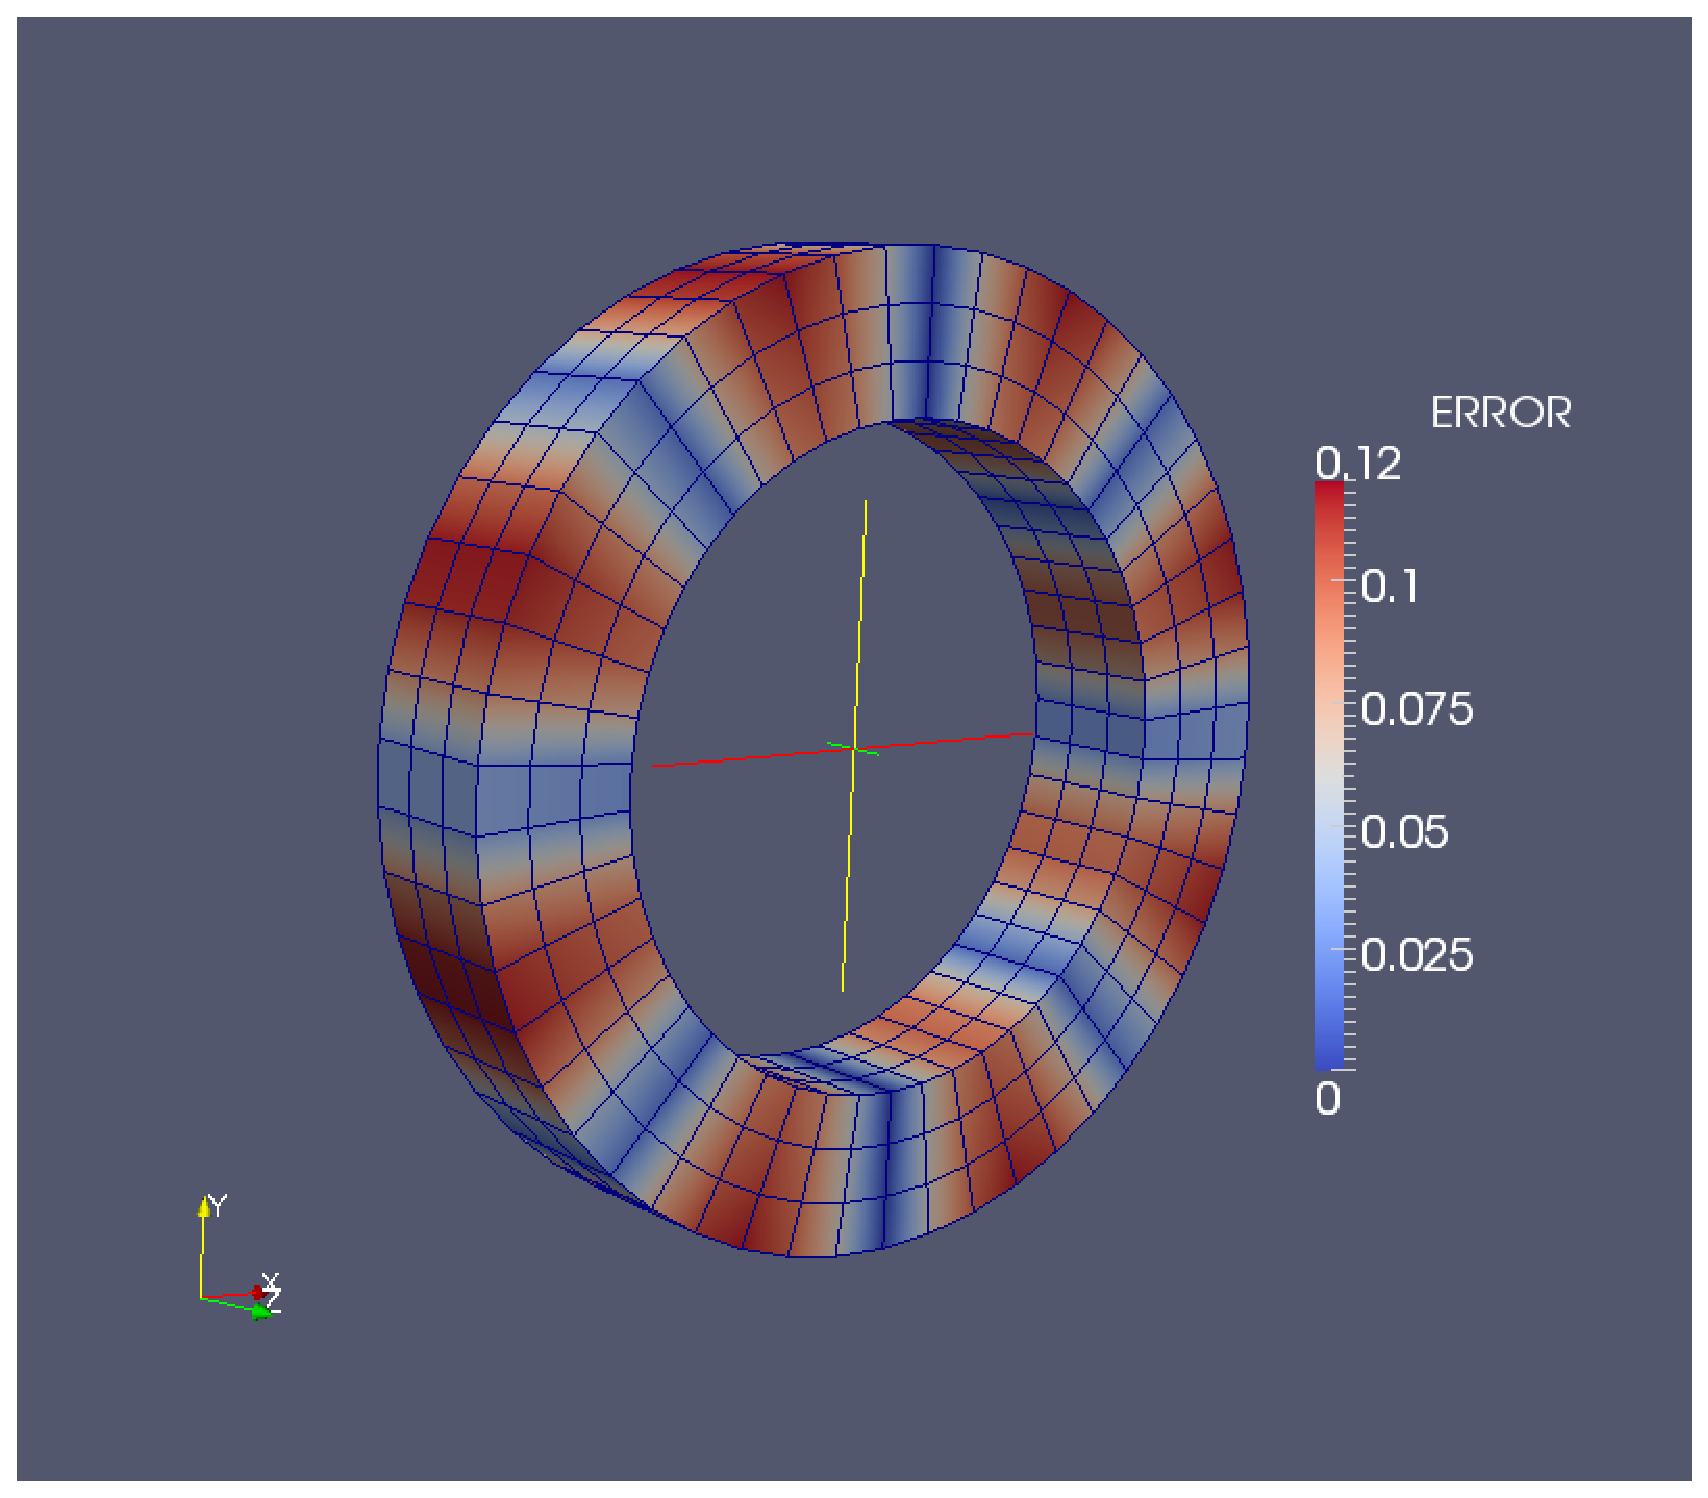
\includegraphics[width=80mm]{RingProjLieNo.eps}}
    \subfigure[]{
      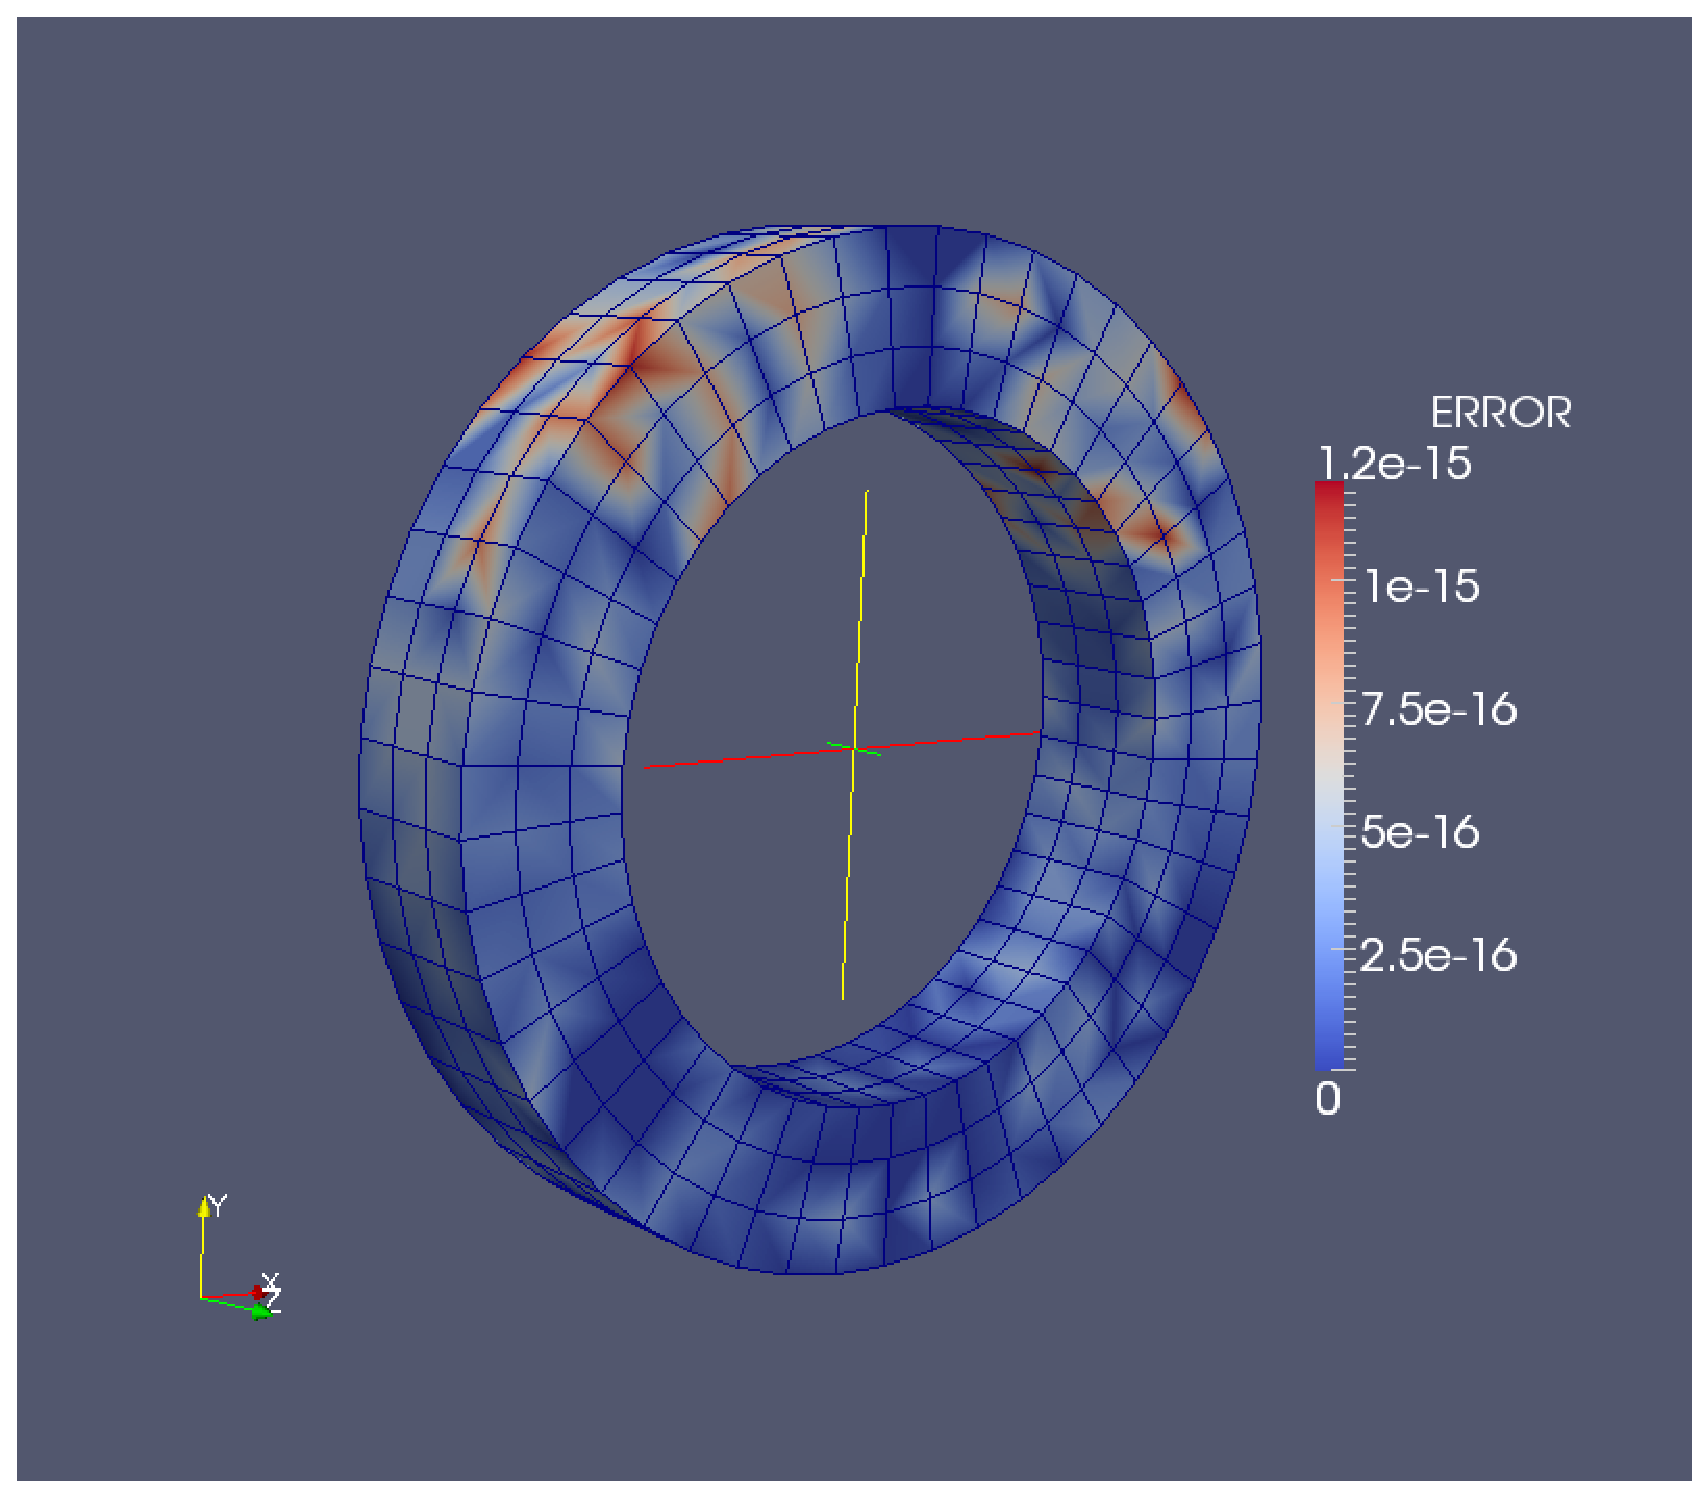
\includegraphics[width=80mm]{RingProjLieHALF.eps}}
    \subfigure[]{
      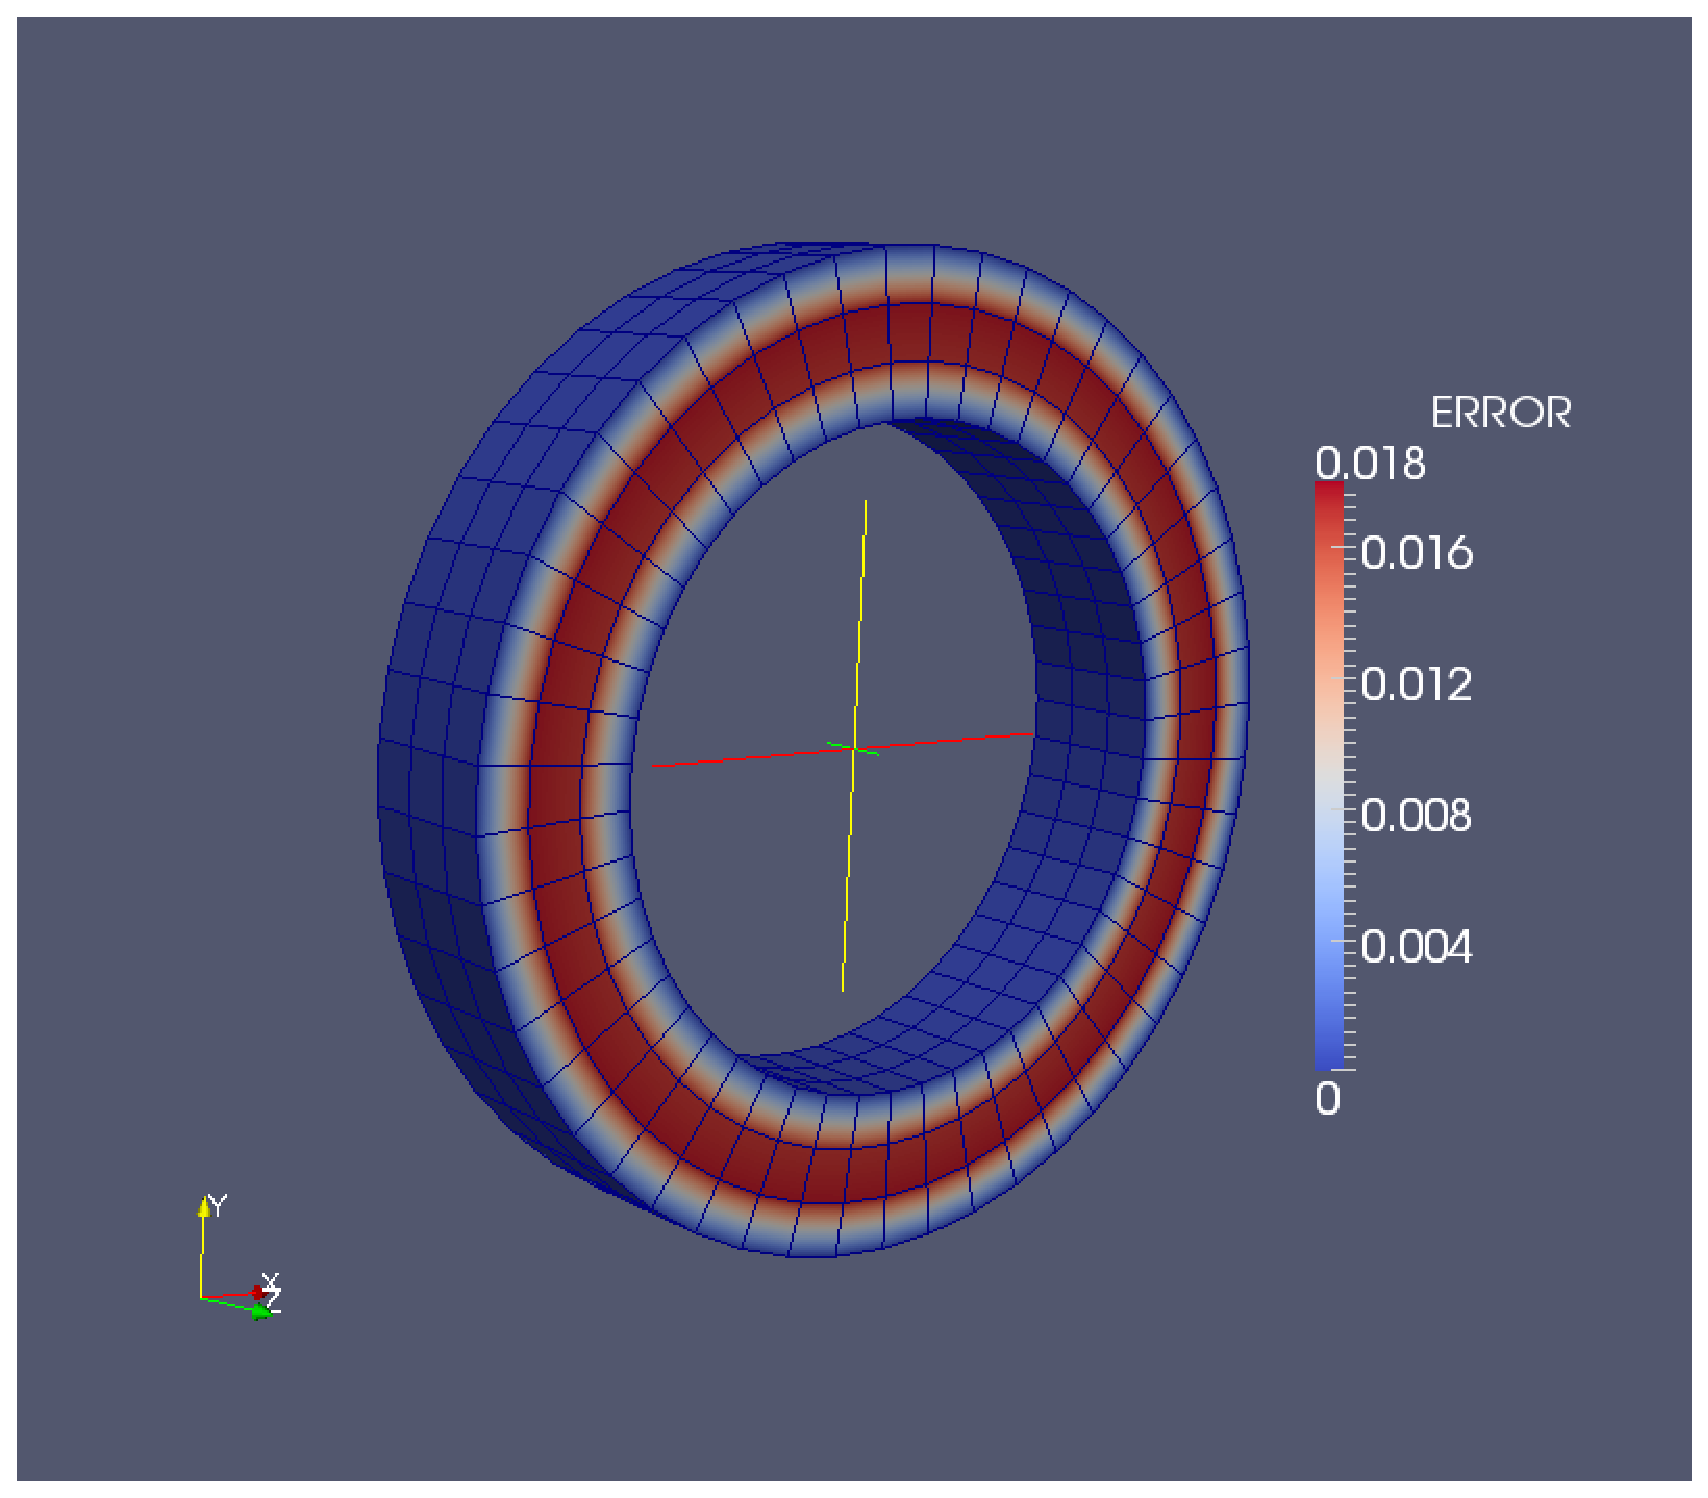
\includegraphics[width=80mm]{RingProjLieFULL.eps}}
    \caption{Frobenius norm of the difference between the deformation
      gradient defined in \eqref{eq:DeformGrad} and the interpolated
      one obtained by polynomial interpolation (a) without Lie
      algebra, (b) with rotation transformed from SO(3) to so(3) and
      (c) with both rotation and right stretch tensor transformed to
      the corresponding Lie algebra .}
    \label{fig:ExampleRing}
  \end{center}
\end{figure}

Figure \ref{fig:ExampleRing}(b) shows a significant improvement on
accuracy when polynomial interpolation is performed in conjugation
with a proper Lie algebra.  In this example, the same interpolation
procedure is repeated. The only exception is that the polynomial
interpolation of the rotation part of the deformation gradient is now
conducted on the Lie algebra rather than on the Lie group itself, as
discussed in the previous section.  This treatment enables the
addition operation of the rotation data and thus legitimate the
polynomial interpolation. The resultant interpolation error of the Lie
algebra method reduces the maximum error by 13 orders of
magnitude. This negligible error demonstrates that the the remapping
with Lie algebra transformation is accurate even if the source and
target mesh are profoundly different in size.

Notice that, however, if the logarithmic mapping is applied to both
the right stretch tensor and the rotation part of the deformation
tensor, then the maximum value of the interpolation error becomes
$0.018$, which falls in between the interpolation errors of the two
cases discussed above, as shown in Figure \ref{fig:ExampleRing}
(c). In this case, the interpolation of deformation gradient on the
middle axis does not perform as good as the interpolation on the inner
and outer surfaces of the annulus. This is due to the fact that the
right stretch tensor varies linearly along the $Y$ direction as shown
in \ref{eq:PolarDecomposition} and thus the direct linear
interpolation performed on the Lie group is capable of reproducing the
exact linear right stretch tensor field while the linear interpolation
performed on Lie algebra cannot. This example demonstrates that there
is hardly any golden rule on how internal variables should
interpolate. The appropriate choice of the interpolation strategy
depends on the situations and the prior knowledge one may acquire and
take advantage of.

\subsubsection{Refinement Study}
To investigate the relation between the mesh refinement and the
overall accuracy of the interpolation, we conduct a refinement study
to obtain the convergence rate and accuracy of the three interpolation
strategies mentioned above. In particular, the error measured by the
Frobenius norm of the interpolated tensor field $\bA$ is numerically
integrated over the entire domain at a variety of refinement levels,
i.e.,
\begin{equation}
  E_{\bA}^{h} =   \int_{B} ||\bA^{exact} (\bX)- \bA^{h}(\bX) ||_{F}  dV  
  \approx \sum^{nen}_{j=1}\sum^{N}_{i=1} ||
    \lambda_{\alpha} (\bxi_{i}) \bA_{\alpha} -
  A^{exact}(\bxi_{i}) ||_{F} \;
  w(\bxi_{i})  J(\bxi_{i}) 
  \label{eq:FrobeniusNormOverall}
\end{equation}
where $\bA$ can be $\bF, \bR, \bU$ and $E_{\bA}^{h}$ is the error
corresponding to the interpolated second order tensor field $\bA$;
$\bxi$ is the Gauss point in the parent domain; $w(\bxi)$ and
$J(\bxi)$ is the weight of the Gauss quadrature and the Jacobian
determinant of the isoparametric mapping at the Gauss points; $N$ is
the number of Gauss points per element and $nen$ is the number of
elelemts in the mesh.

The refinement study uses the same bending problem described
before. Initially, the domain of the size $L \times L/16 \times L/16$
is meshed by 4 elements along the $X$ direction and 1 element along
the $Y$ and $Z$ directions. The aspect ratio of all element are
therefore 4. Then, we refine the mesh by increasing the number of
element linearly in both $X$ and $Y$ direction, but discretize $Z$
direction with only one element.  In each refined mesh, the aspect
ratio, length/width, remains constant for all elements.
\begin{figure}[htbp]
  \begin{center}
    \unitlength=1.0mm
    \subfigure[]{
      \includegraphics[width=80mm]{RefinementF.eps}}
    \subfigure[]{
      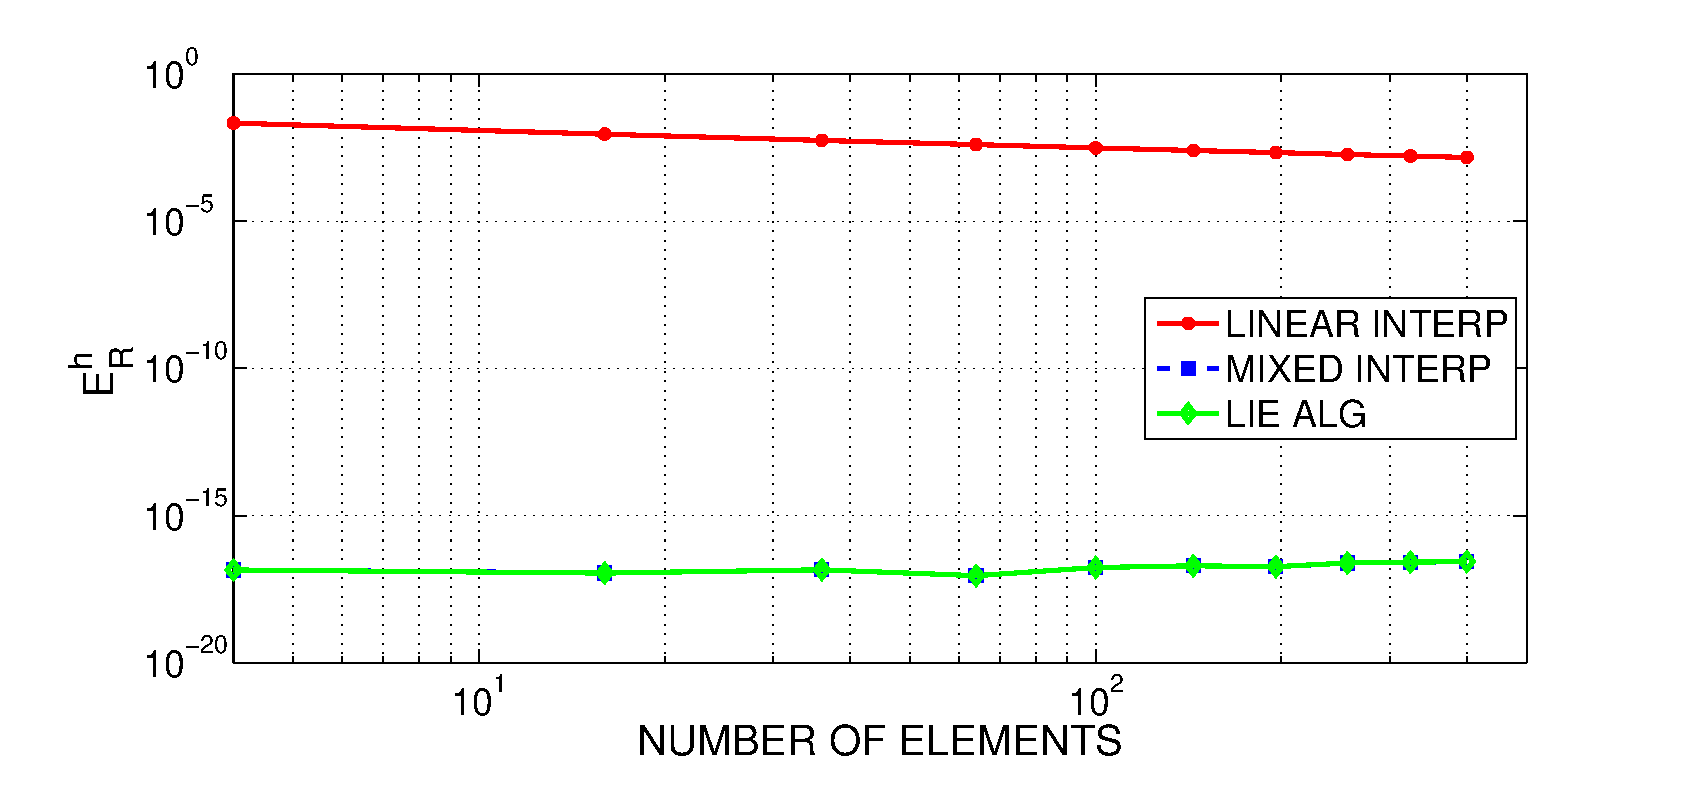
\includegraphics[width=80mm]{RefinementR.eps}}
    \subfigure[]{
      \includegraphics[width=80mm]{RefinementU.eps}}
    \caption{Convergence plots for the annulus bending problem: errors
      of (a) deformation gradient, (b) rotation and (c) right
      stretch.}
    \label{fig:RingRefinement}
  \end{center}
\end{figure}

Figures \ref{fig:RingRefinement}(a)-(c) show the convergence curves
obtained via all three schemes.  The errors of the deformation gradient,
rotation and right stretch tensor are computed with mesh of different 
sizes. Each plot collects three curves, corresponding to the standard 
polynomial interpolation (red), the polynomial interpolation conducted on 
Lie algebra of both the rotation and right stretch (green) and a mixed approach in which stretch is
linearly interpolated and rotation is interpolated via Lie algebra
(blue).  As evident from the convergent plots, the rate of convergence
obtained via the Lie algebra is faster than the standard interpolation
approach. The Lie algebra approach also exhibits higher accuracy in
coarse mesh. However, as demonstrated in the previous example, the
linear interpolation of stretch is less accurate when conducted on Lie
algebra than in the Lie group due to the linearity of the stretch
field as expressed in \eqref{eq:RightPolar}. This linearity causes the
error of the interpolated deformation gradient being within the
machine error if the mixed approach is used, but also leads to error
when attempting to reproducing linear field with the logarithmic
mapping scheme. The resultant convergence rate of stretch field is
approximately the same as that of the deformation gradient --the error
measured by the Frobenius norm reduces by roughly two orders when the
number of elements increased by two orders.

On the other hand, the interpolation of rotation on $so(3)$ exhibits
only machine error. This can be explained by the fact that the
rotation described in $so(3)$ actually varies linearly with respect to
$X$ as the rotation angle $X/R$ varies linearly with respect to
$X$. Therefore, when the linear rotation is interpolated in $so(3)$
linearly, the interpolation recovers the exact solution. Meanwhile,
the convergence rate is very slow if the interpolation is performed
directly on the $SO(3)$. The error of rotation only reduces less than
one order when the number of the elements is increased 100 times.

\subsubsection{Comparisons with Other Internal Variable Recovery Schemes}
To compare the performance of the proposed internal variable recovery procedure
with other commonly used numericla scheme, we assign the analytical solution of 
the deformation field at the Gauss points of the 16-element coarse mesh and project 
it to the node by a variety of recovery methods. The errors defined in 
\eqref{eq:FrobeniusNormDistribution} and \eqref{eq:FrobeniusNormOverall} 
are both computed. 

Six internal variable recovery procedures are compared in  Table 
\ref{tab:RingErrorComparison}. The first method (labeled as direct averaging) 
employs a searching scheme to determine the closest Gauss points to a node 
in each element. The value of the closest Gauss point is assigned
to the node. If the same node is shared by more than one element, then the 
Gauss point values are averaged among the Gauss points that shared the same node
 in different elements. In the  extrapolation approach, we establish shape functions 
 using Gauss points as local node, then extrapolate Gauss point data to the actual node of each finite 
element. The nodal values are then averaged element-wise in a similar fashion of 
the first method. The next two approaches both employ the variational projection
operator globally. The only difference between the two is that one projects the polar 
decomposed deformation field and another one projects the deformation field directly 
without polar decomposition. The last two approach projects the polar decomposed 
rotation and right stretch tensor field globally with variational projection operators. 
While both of them  transfer the rotation field from $SO(3)$ to $so(3)$, only the second last 
approach (denoted as full Lie Alg) transfer the right stretch tensor from $GL(3)$ to $gl(3)$.  
 
\begin{table}[htbp]
  \begin{center}
    \begin{tabular}{ l l l }
      \toprule
      
      Method
      &
      Range of $e^{h}(\bX)$
      & 
      Global Error $E_{F}^{h}$
      \\
      \hline
      Direct Averaging
      &
      $0.063-0.14$
      & 
      $0.0012$
      \\
      Extrapolation   
      &
      $0.066-0.70$
      &
      $0.0071$
      \\
      Variational Projection (with SVD)  
      &
      $0.017-0.02$
      & 
      $2.8 \times 10^{-5}$
      \\
       Variational Projection (w/o SVD)  
      &
      $0.017-0.02$
      & 
      $2.8 \times 10^{-5}$
      \\
       Variational Projection (full Lie Alg)  
      &
      $0.0078-0.0087$
      & 
      $2.6 \times 10^{-17}$
      \\
      Variational Projection (mixed)  
      &
      $5.4 \times 10^{-16} - 2.4 \times 10^{-13}$
      & 
      $3.3 \times 10^{-17}$
      \\
      \bottomrule
    \end{tabular}
    \caption{Comparison of various internal variable recovery methods 
                  for the bending annulus problem.}
    \label{tab:RingErrorComparison}
  \end{center}
\end{table}

Table \ref{tab:RingErrorComparison} demonstrates that the four variational 
projection cases produce less error than both the direct averaging and 
extrapolation methods regardless of whether Lie algebra is employed. 
This result is consistent with the proposition in section 2 where the 
variational operators are proved to minimize the L2 norm and thus 
provides further evidence of the superior accuracy of the variational 
projection method. Furthermore, the global error measured by the $E^{h}_{F}$ 
is reduced by 12 order when the rotation interpolation is conducted in $so(3)$ 
instead of $SO(3)$. Even though the $e^{h}(\bX)$ appears to be lower in mixed 
approach, this reduction in global error is within the same order.   


\subsection{Elastic-Plastic Upsetting of an Axisymmetric Billet}
This example demonstrates the outstanding ability of the variational
transfer operator to project internal variables onto the admissible
space. We integrate the variational projection operator and the Lie
algebra interpolation techniques in a framework where variational
projection operator is used in conjugation with logarithmic mapping.
The calculation we conducted is proposed as a severe test problem by
\citet{Krieg.Krieg:1977}, \citet{Taylor.Becker:1983} and
\citet{Simo.Hughes:1998}. For completeness, we briefly review the
problem statement below.

Consider a cylindrical billet with initial radius = $10mm$ and initial
height = $30mm$. Due to symmetry with respect to the three Cartesian
axes, only $1/8$ of the specimen is considered. The top boundary of
the reference configuration is fixed by a roller such that it does not
move vertically but is free to expand horizontally. The bottom of the
reference configuration is fixed horizontally, but is prescribed a
vertical displacement.  The constitutive response of the specimen is
simulated via a J2 elasto-plastic model with linear isotropic
hardening. The material parameters used in this study is identical
with those in are listed in \citep{Taylor.Becker:1983} and
\citep{Simo.Hughes:1998} (see Table \ref{tab:UpsetBillet}).
\begin{table}[htbp]
  \begin{center}
    \begin{tabular}{ l l }
      \toprule
      
      Young's modulus
      &
      $E = 1000$MPa
      \\
      Poisson's ratio
      &
      $\nu = 0.3$
      \\
      Yield stress  
      &
      $\sigma_{y} = 1.00$MPa
      \\
      Hardening modulus   
      &
      $H=3.0$MPa
      \\
      \bottomrule
    \end{tabular}
    \caption{Material parameters for the stainless steel.}
    \label{tab:UpsetBillet}
  \end{center}
\end{table}

Four finite element simulations are performed and compared against the
published results in \citep{Krieg.Krieg:1977, Taylor.Becker:1983,
  Simo.Hughes:1998}.  To preserve the radial symmetry of the cylinder,
the hexahedral mesh is generated via a radial meshing algorithm in a
mesh generation software called CUBIT such that node distribution is
unbiased along the radial direction. The 8-node and 27-node Lagrange
hexahedral elements are both used on two meshes consisting of 693 and
2175 elements. The final configurations in all four simulations are
attained in 120 equal steps. Figure \ref{fig:LoadDeflection} shows the
resulting load-deflection curves. Both results obtained from 8-node
and 27-node element are in good agreement with
\citep{Krieg.Krieg:1977, Taylor.Becker:1983, Simo.Hughes:1998}.
\begin{figure}[htbp]
  \begin{center}
    \unitlength=1.0mm
      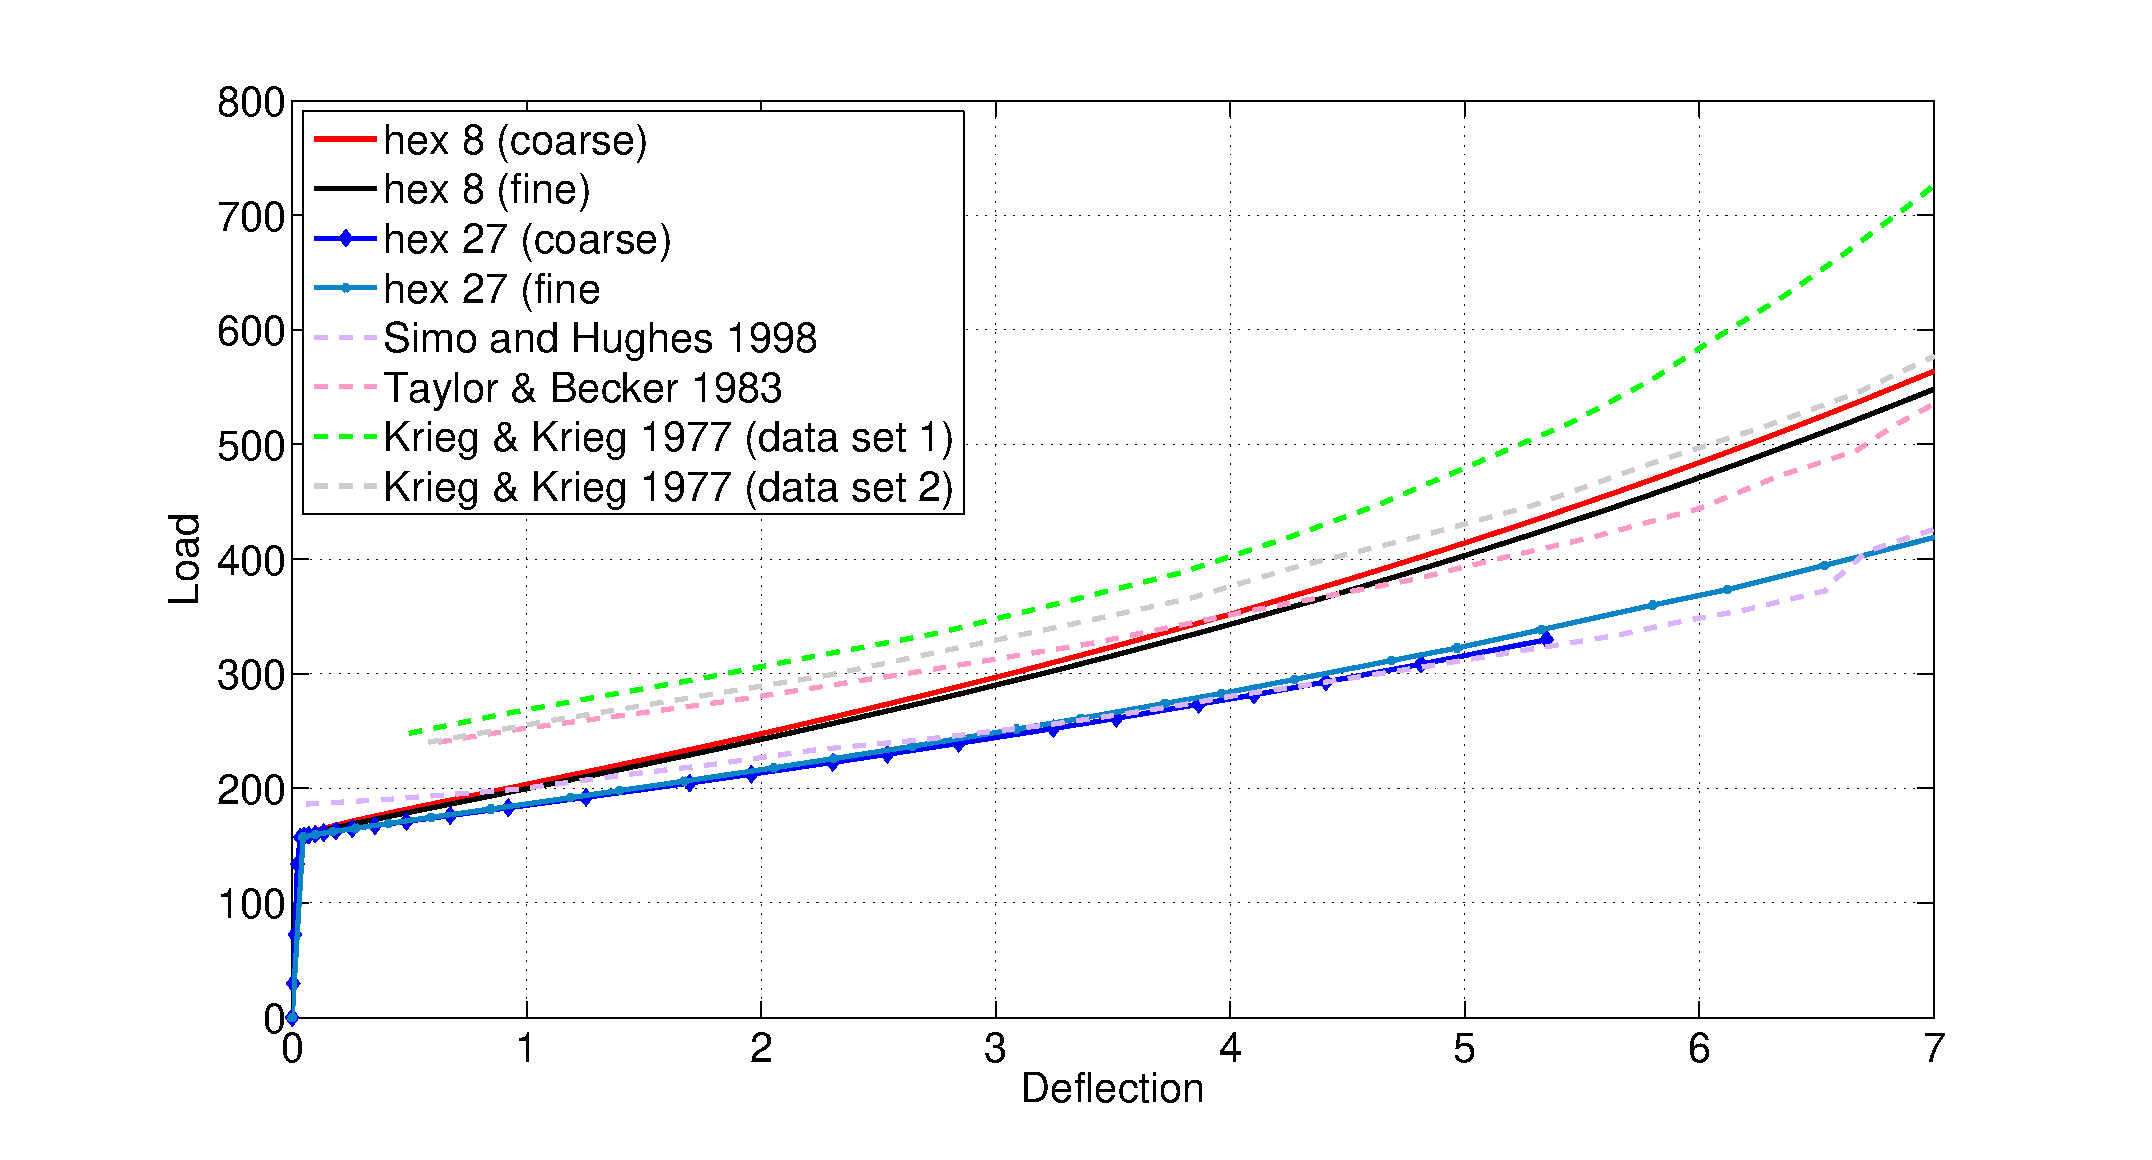
\includegraphics[width=160mm]{Load_Deflection.eps}
      \caption{Load-deflection curve of the elastic-plastic upsetting
        of an axisymmetric billet problem. }
    \label{fig:LoadDeflection}
  \end{center}
\end{figure}

\subsubsection{Admission Range of Isochoric Plastic Response}
At each time step throughout the simulations, the plastic split of the
deformation gradient $\bF^{p} = (\bF^{e})^{-1} \cdot \bF$ is stored.
Figure \ref{fig:BilletNOLie} illustrates two projections of $\bF^{p}$
calculated from the Gauss points of the two 8-node finite element
meshes through standard Galerkin projection, without the application
of Lie algebra. The color in Figure \ref{fig:BilletNOLie} represents
the determinant of $\bF^{p}$ and the deformed mesh is extracted from
the last time step with $53\%$ upsetting.

Ideally, the plastic deformation of the material obeying J2 plasticity
must be isochoric, as the plastic flow direction is
isochoric. However, our results indicate that this is not necessarily
the case when projection is conducted without transforming $\bF^{p}$
to the corresponding Lie algebra. Since linear interpolation is only
legitimate when addition operator is valid, which is not the case for
$F^{p}$, projections conducted directly on $\bF^{p}$ might cause the
projected $\bF^{p}$ is not being admissible to the special linear
group. Consequently, a spurious volumetric plastic deformation is
created if one attempting to directly project $\bF^{p}$ from Gauss
points to nodal points for interpolations. This spurious volumetric
plastic deformation caused by inappropriate projection is depicted in
Figures \ref{fig:BilletNOLie}(a) and (b).

The determinant of the plastic split of the projected deformation
gradient ranges from 0.83 to 1.24 in the coarse mesh, and from 0.64
and 1.40 in the fine mesh at $53\%$ upsetting. This severe error
occurs when significant amount of distortion of mesh accumulated at
the edge of the bottom face, as shown in Figure
\ref{fig:BilletNOLie}(a). Remarkably, the spurious plastic volumetric
strain had not been eliminated through refinement, as the distortion
of the finite element mesh is inevitable regardless of the mesh size.
\begin{figure}[htbp]
  \begin{center}
    \unitlength=1.0mm
    \subfigure[]{
      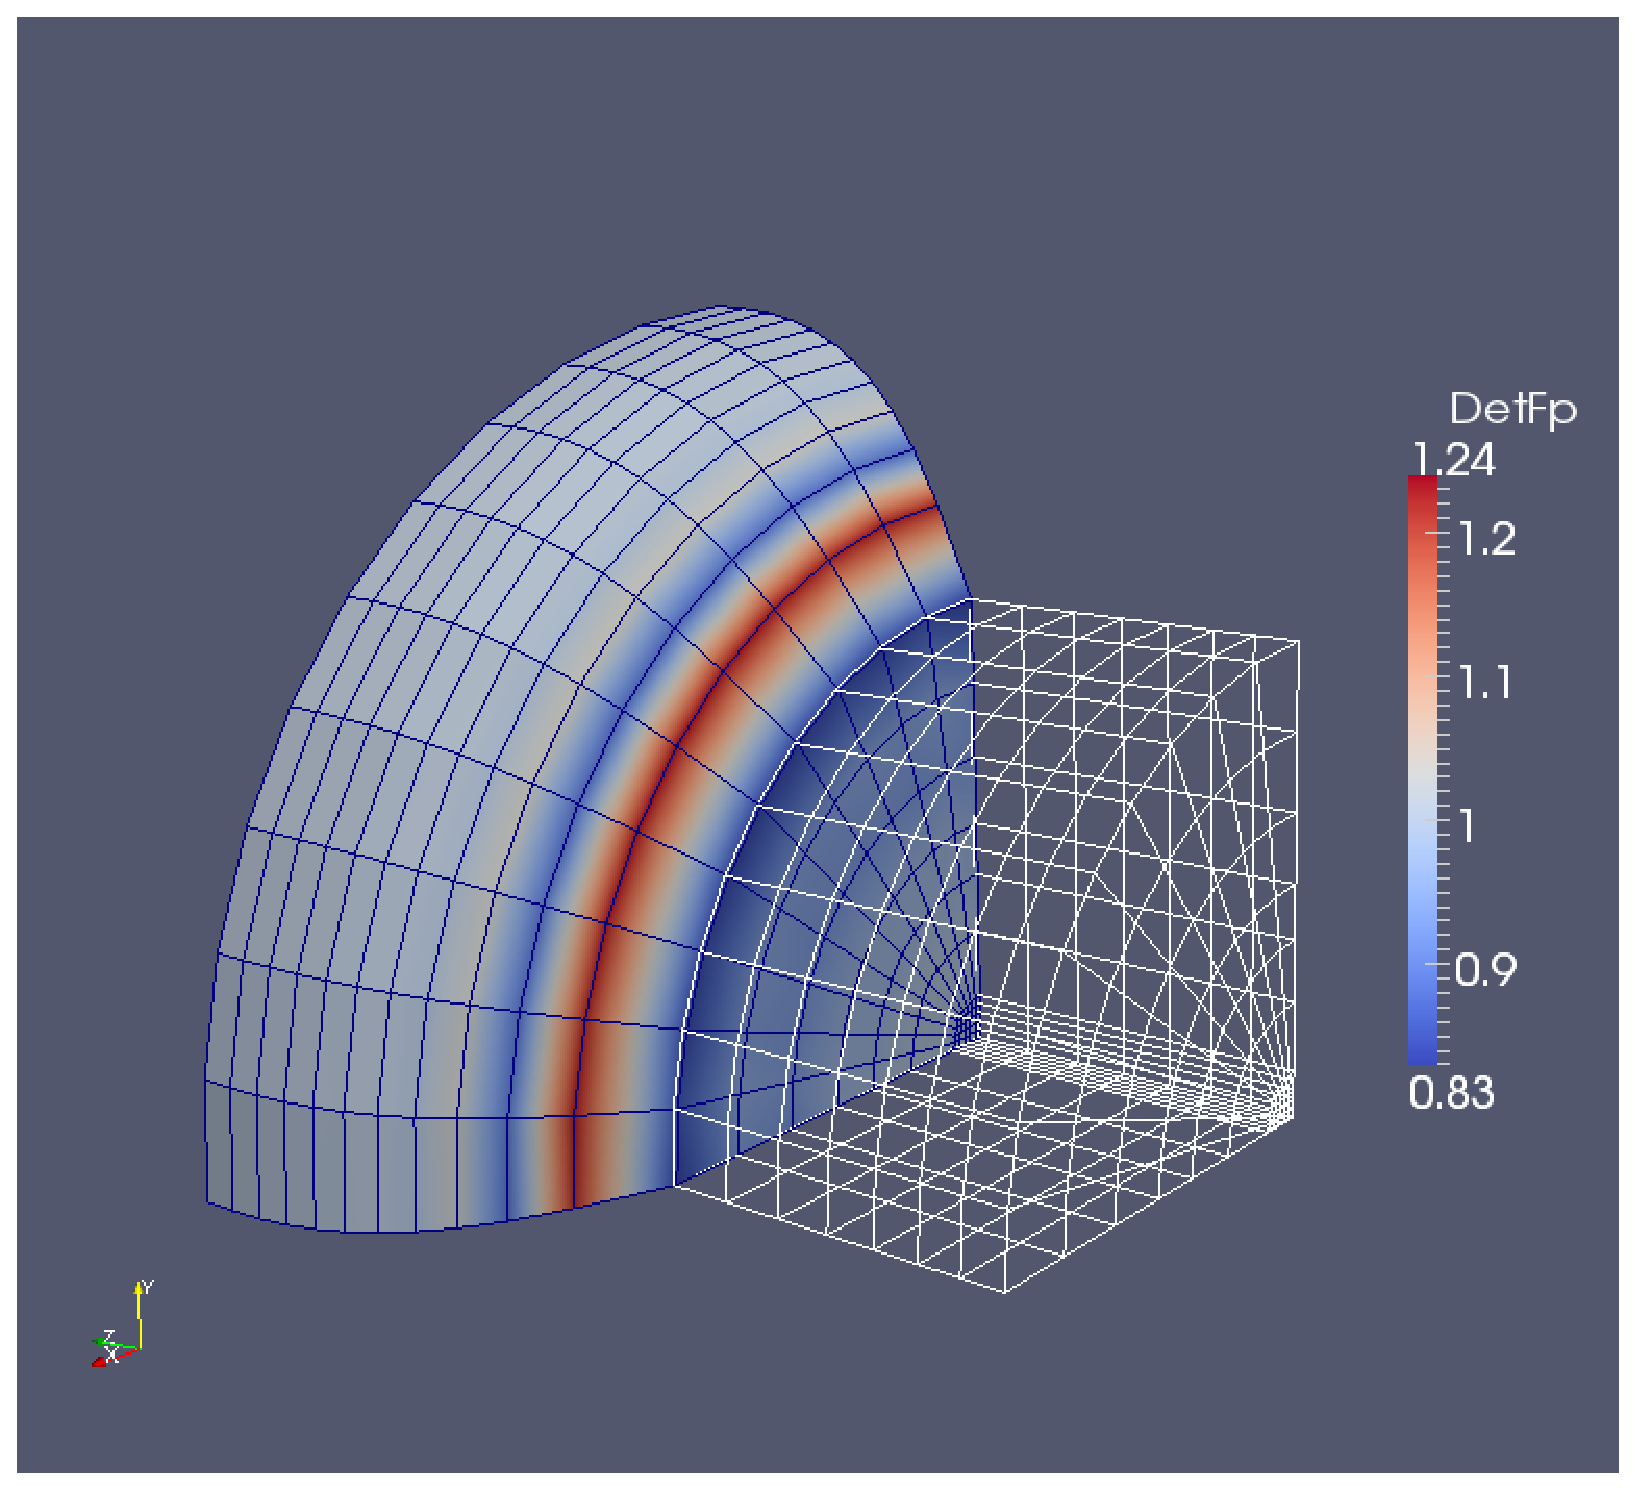
\includegraphics[width=80mm]{HEX8medium_DIRECT_woLie.eps}}
    \subfigure[]{
      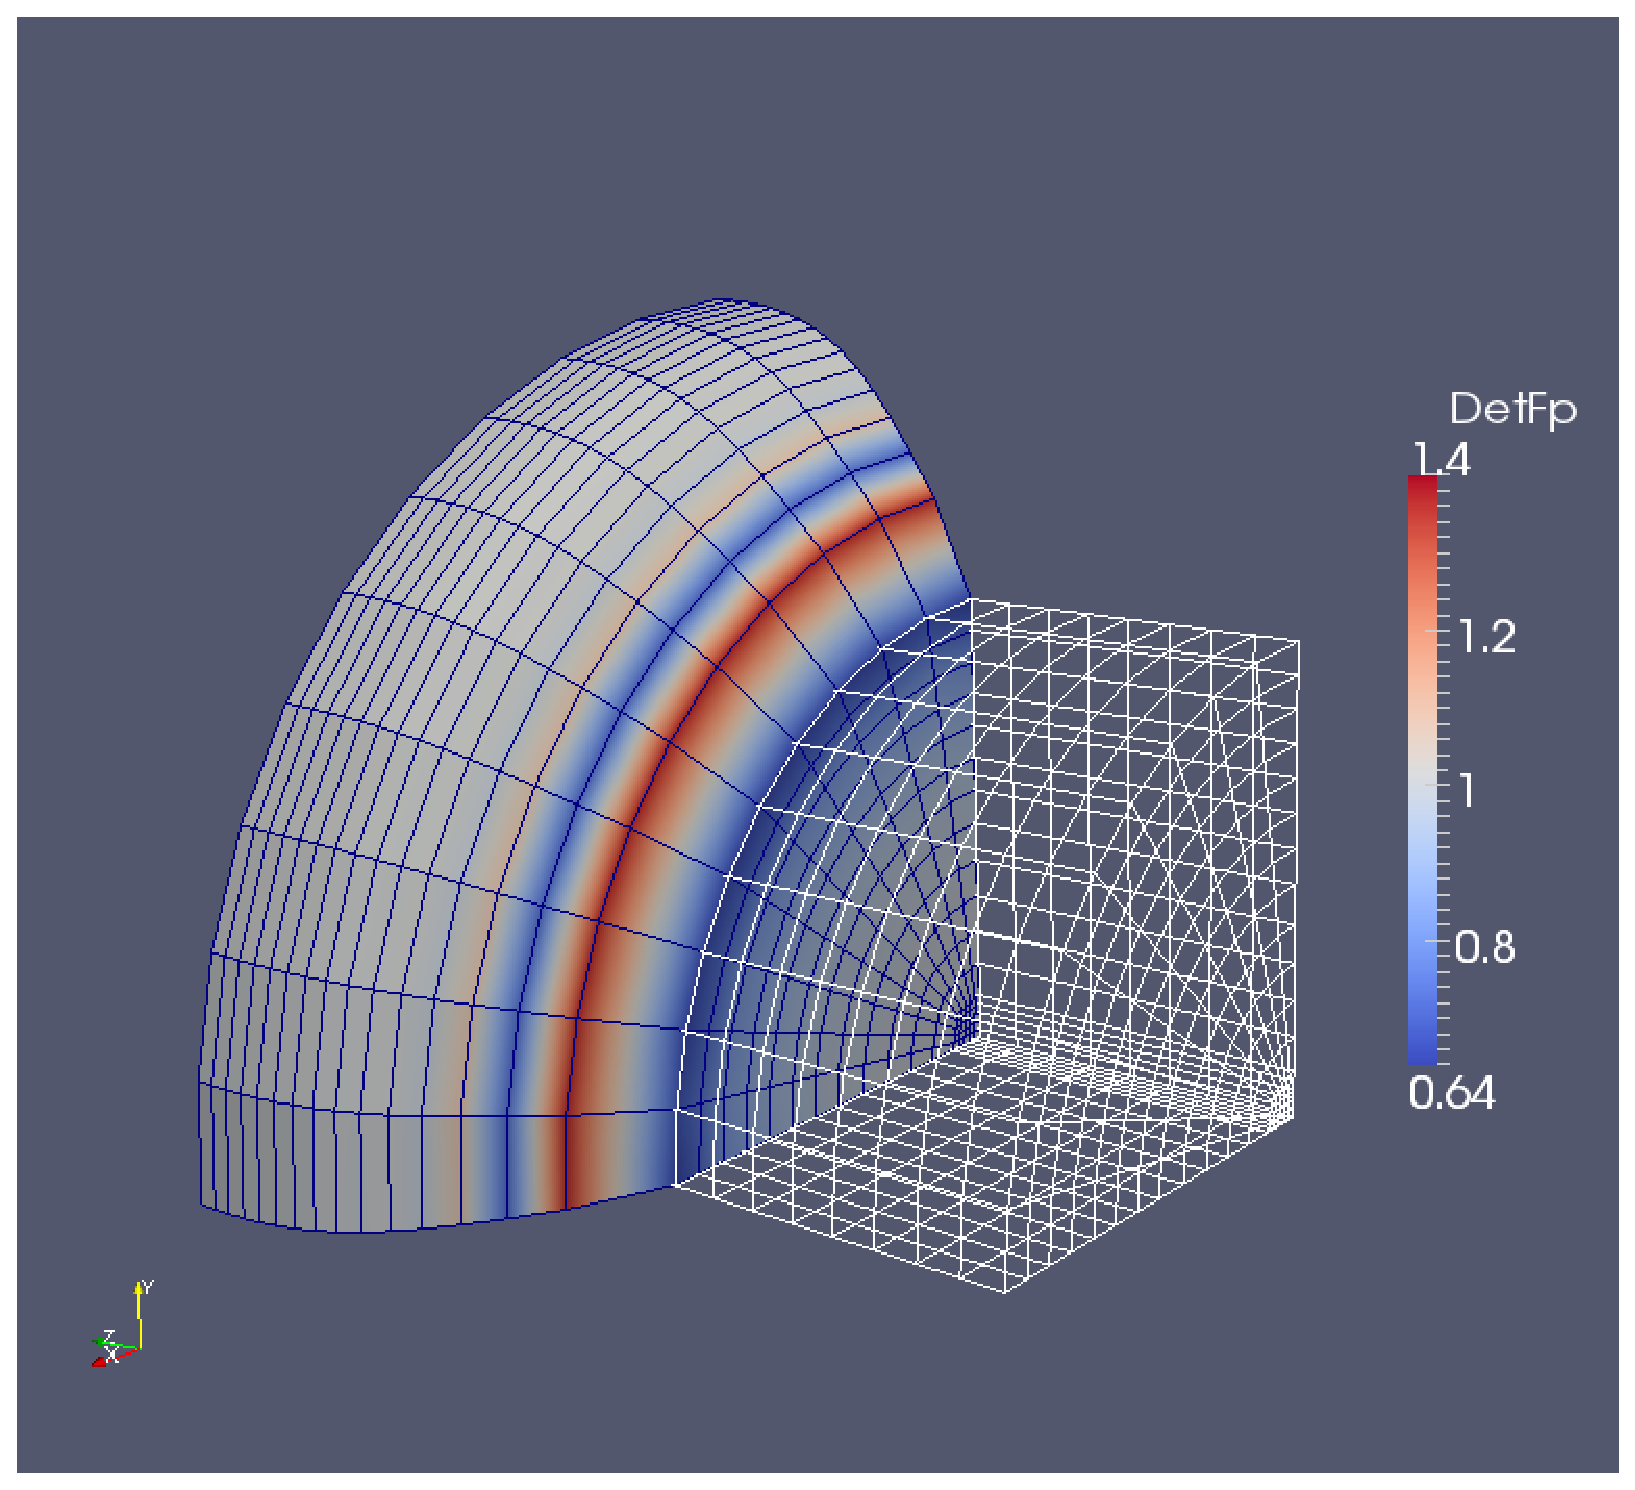
\includegraphics[width=80mm]{HEX8fine_DIRECT_woLie.eps}}
    \caption{The plastic split of the deformation gradient projected
      on deformed meshes with (a) 693 and (b) 2175 hexahedral finite
      elements. Projections are conducted without transformation
      between Lie group and Lie algebra.}
    \label{fig:BilletNOLie}
  \end{center}
\end{figure}

If the projection of the plastic split $\bF^{p}$ is conducted through
Lie algebra, then the resultant projected plastic split remains
isochoric as illustrated in Figure \ref{fig:BilletNOLie}(b).  The
projected plastic split field shown in Figure \ref{fig:BilletNOLie}(b)
is obtained through the following procedure.  First, $F^{p}$ is
decomposed into rotation and right stretch tensors through singular
value decomposition.  Then, the rotation tensor is mapped from $SO(3)$
into $so(3)$ and the stretch is mapped from $GL^{+}(3)$ to $gl(3)$.
By applying \eqref{eq:ProjectionZ} on $so(3)$ and $gl(3)$ where
addition operation is valid, the projected field is guaranteed to
remain in the admissible space. The projected fields are then
transformed back from Lie algebra $so(3)$ and $gl(3)$ back to $SO(3)$
and $GL(3)$ at nodes and the projected plastic split field is
obtained by interpolating $\bF = \bR \cdot \bU$ at nodes of the finite
element mesh. Results obtained from the calculation show that the
determinant of the projected plastic split is 1 everywhere in the
finite element domain and hence there is no spurious dilation and/or
contraction created due to projection from Gauss points to nodes. This
feature help preventing non-physical data injected into the simulation
when remeshing and/or post-processing take place. As indicated in
Figure \ref{fig:BilletNOLie}(b), this constraint-preserving feature
holds regardless of mesh size.

\begin{figure}[htbp]
  \begin{center}
    \unitlength=1.0mm
    \subfigure[]{
      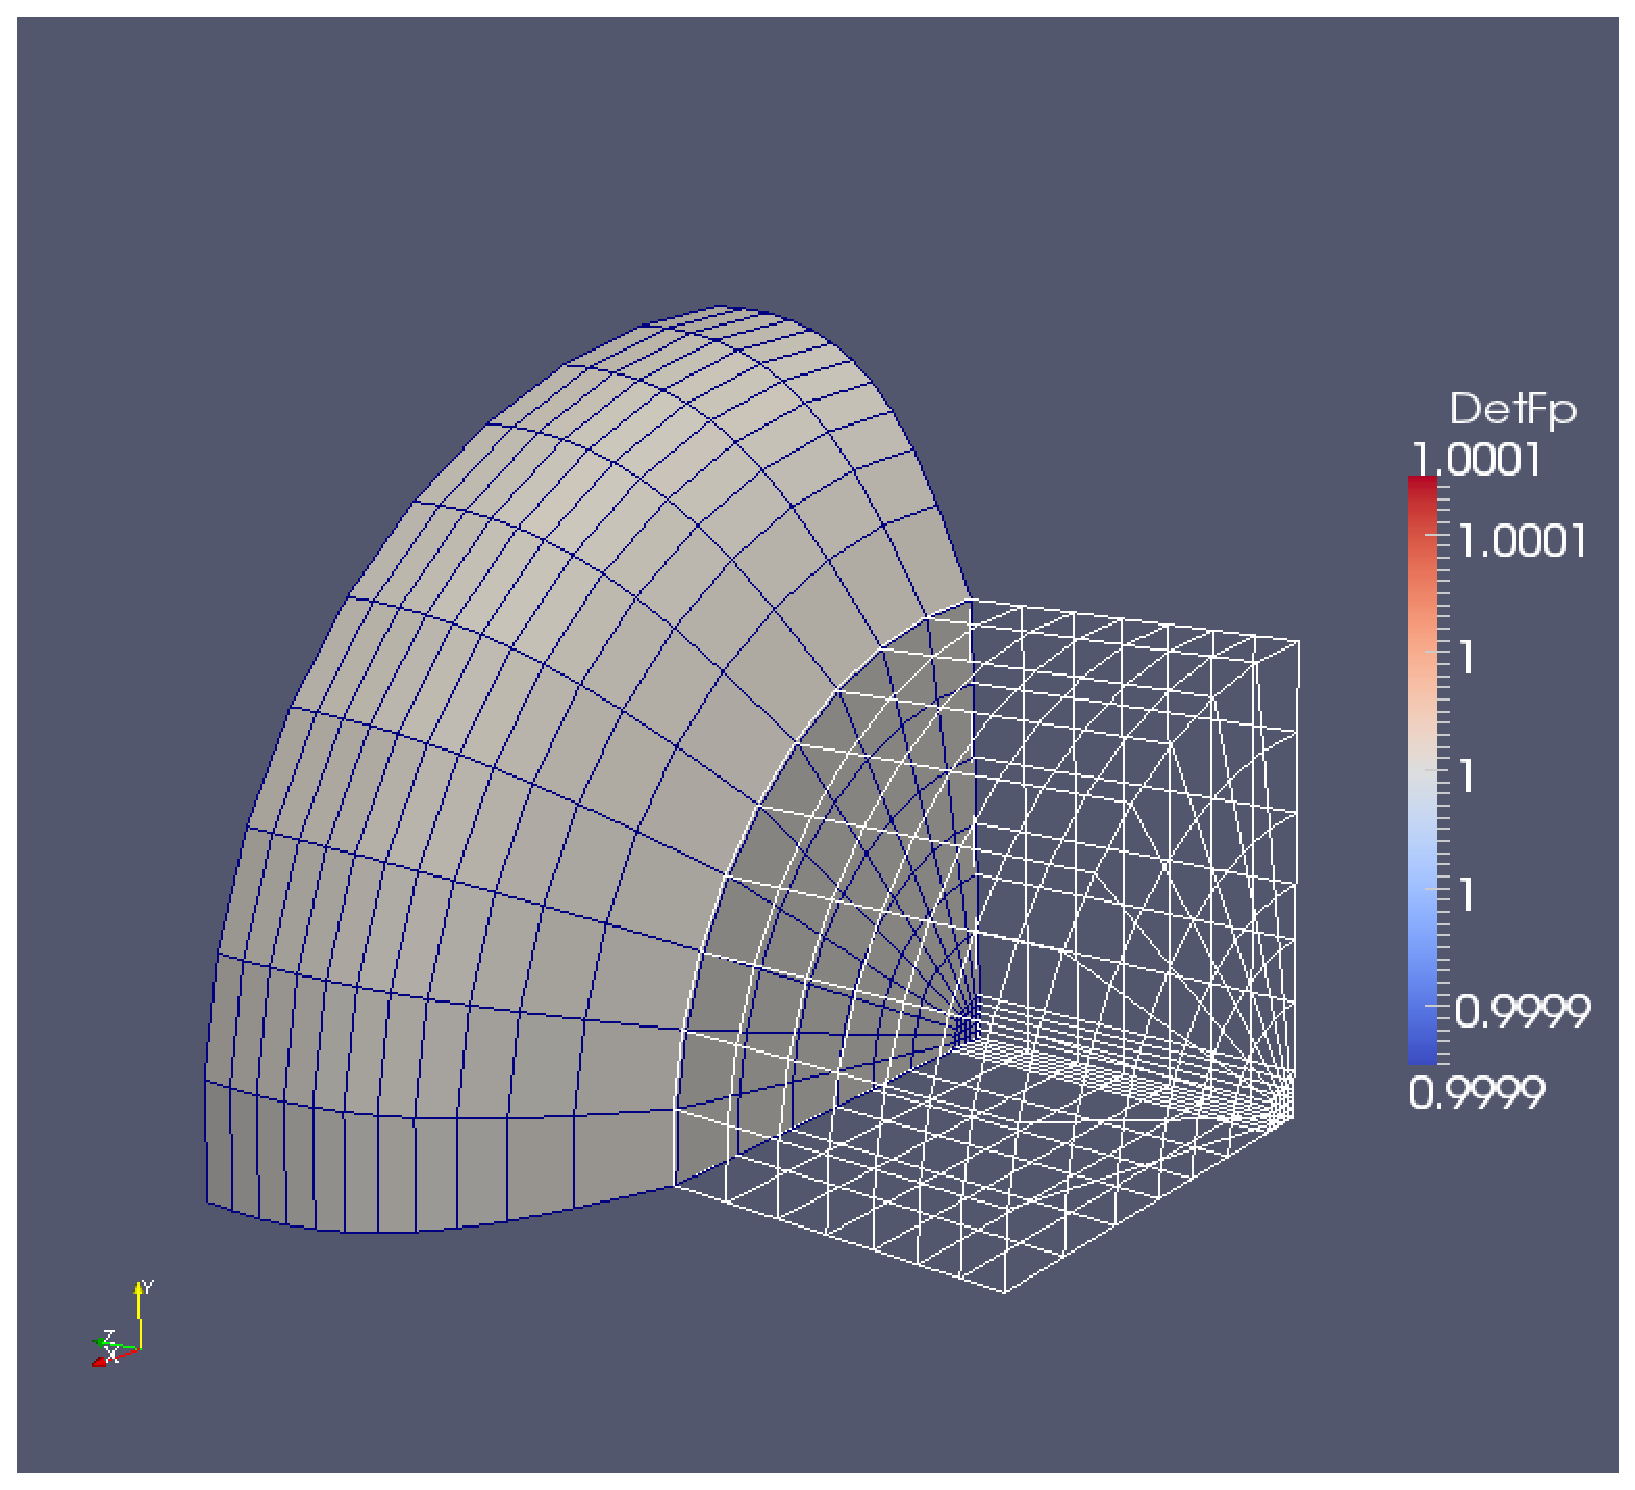
\includegraphics[width=80mm]{HEX8medium_DIRECT_wLie.eps}}
    \subfigure[]{
      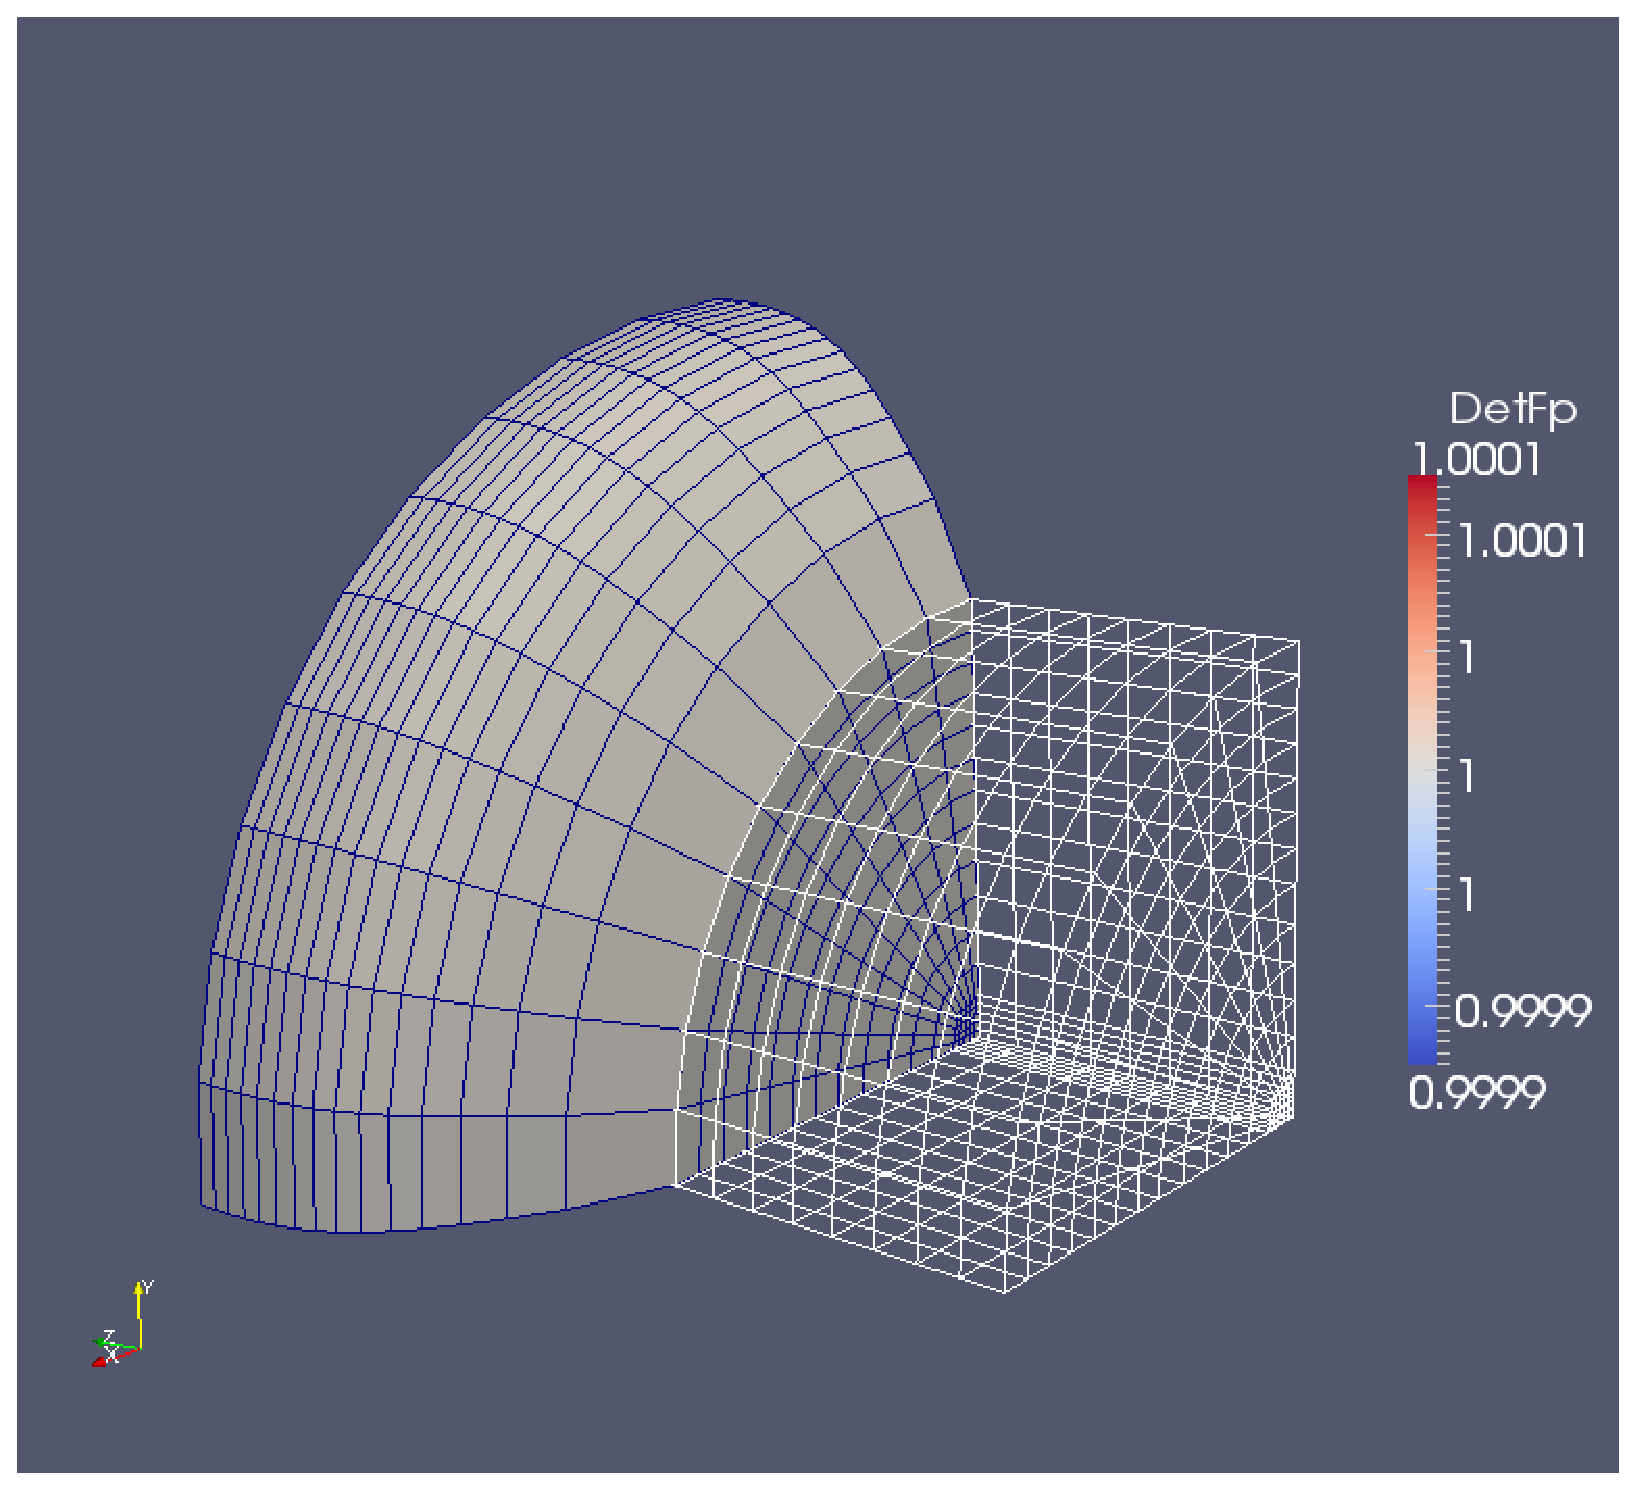
\includegraphics[width=80mm]{HEX8fine_DIRECT_wLie.eps}}
    \caption{The plastic split of the deformation gradient projected
      on deformed meshes with (a) 693 and (b) 2175 hexahedral finite
      elements. Projections are conducted with transformation between
      Lie group and Lie algebra.}
    \label{fig:BilletWLie}
  \end{center}
\end{figure}

\subsubsection{Comparisons with Other Internal Variable Recovery Schemes}
We compare the performance of the same set of internal variable recovery schemes 
again using the upsetting billet example. Here the Gauss points of the coarse mesh 
is first projected to the node. Using the nodal values and the interpolation functions, 
we compute the nodal value of $\det(\bF^{p})$ and the errors defined in 
\eqref{eq:FrobeniusNormOverall}.  Table \ref{tab:BilletErrorComparison} demonstrates 
the properties of the projected plastic deformation. Among the six internal variable recovery 
approaches, only the ones applying Lie algebra is able to preserve the isochoric property of 
the J2 model. Since the mesh with 693 element used in this comparison study is 
relatively fine, the difference in global error is not significant. Nevertheless,  the variational projections 
are still the more accurate approaches among all the recovery procedures.  
 
 \begin{table}[htbp]
  \begin{center}
    \begin{tabular}{ l l l }
      \toprule
      
      Method
      &
      Range of $\det(\bF^{p})$
      & 
      Global Error $E_{F}^{h}$
      \\
      \hline
      Direct Averaging
      &
      $1-1.25$
      & 
      $9.35 \times 10^{-9}$
      \\
      Extrapolation   
      &
      $0.95-1.1$
      &
      $1.56 \times 10^{-8}$
      \\
      Variational Projection (with SVD)  
      &
      $0.89-1.1$
      & 
      $7.36 \times 10^{-9}$
      \\
       Variational Projection (w/o SVD)  
      &
      $0.83-1.24$
      & 
      $7.4017 \times 10^{-9}$
      \\
       Variational Projection (full Lie Alg)  
      &
      $1$
      & 
      $7.07 \times 10^{-9}$
      \\
      Variational Projection (mixed)  
      &
      $1$
      & 
      $7.37 \times 10^{-9}$
      \\
      \bottomrule
    \end{tabular}
    \caption{Comparison of various internal variable recovery methods for the upsetting billet problem.}
    \label{tab:BilletErrorComparison}
  \end{center}
\end{table}

\section{Conclusion}

\bibliographystyle{plainnat}
\bibliography{tomiv}

\end{document}
